%==========================================
%
% Sibgrapi 2012 paper
% John Silva, João Smith, ...
%
%==========================================


% Note that the a4paper option is mainly intended so that authors in
% countries using A4 can easily print to A4 and see how their papers will
% look in print - the typesetting of the document will not typically be
% affected with changes in paper size (but the bottom and side margins will).
% Use the testflow package mentioned above to verify correct handling of
% both paper sizes by the user's LaTeX system.
%
% Also note that the "draftcls" or "draftclsnofoot", not "draft", option
% should be used if it is desired that the figures are to be displayed in
% draft mode.
%
\documentclass[10pt, conference]{IEEEtran}

% *** MISC UTILITY PACKAGES ***
%
%\usepackage{ifpdf}
% Heiko Oberdiek's ifpdf.sty is very useful if you need conditional
% compilation based on whether the output is pdf or dvi.
% usage:
% \ifpdf
%   % pdf code
% \else
%   % dvi code
% \fi
% The latest version of ifpdf.sty can be obtained from:
% http://www.ctan.org/tex-archive/macros/latex/contrib/oberdiek/
% Also, note that IEEEtran.cls V1.7 and later provides a builtin
% \ifCLASSINFOpdf conditional that works the same way.
% When switching from latex to pdflatex and vice-versa, the compiler may
% have to be run twice to clear warning/error messages.






% *** CITATION PACKAGES ***
%
%\usepackage{cite}
% cite.sty was written by Donald Arseneau
% V1.6 and later of IEEEtran pre-defines the format of the cite.sty package
% \cite{} output to follow that of IEEE. Loading the cite package will
% result in citation numbers being automatically sorted and properly
% "compressed/ranged". e.g., [1], [9], [2], [7], [5], [6] without using
% cite.sty will become [1], [2], [5]--[7], [9] using cite.sty. cite.sty's
% \cite will automatically add leading space, if needed. Use cite.sty's
% noadjust option (cite.sty V3.8 and later) if you want to turn this off.
% cite.sty is already installed on most LaTeX systems. Be sure and use
% version 4.0 (2003-05-27) and later if using hyperref.sty. cite.sty does
% not currently provide for hyperlinked citations.
% The latest version can be obtained at:
% http://www.ctan.org/tex-archive/macros/latex/contrib/cite/
% The documentation is contained in the cite.sty file itself.






% *** GRAPHICS RELATED PACKAGES ***
%
%\usepackage{subimages}
%\setfigdir{figs}
\usepackage{epsfig}
\usepackage{epstopdf}
\usepackage{subfigure}
\graphicspath{{./images/}}

% *** MATH PACKAGES ***
%
\usepackage[cmex10]{amsmath}
% A popular package from the American Mathematical Society that provides
% many useful and powerful commands for dealing with mathematics. If using
% it, be sure to load this package with the cmex10 option to ensure that
% only type 1 fonts will utilized at all point sizes. Without this option,
% it is possible that some math symbols, particularly those within
% footnotes, will be rendered in bitmap form which will result in a
% document that can not be IEEE Xplore compliant!
%
% Also, note that the amsmath package sets \interdisplaylinepenalty to 10000
% thus preventing page breaks from occurring within multiline equations. Use:
\interdisplaylinepenalty=2500
% after loading amsmath to restore such page breaks as IEEEtran.cls normally
% does. amsmath.sty is already installed on most LaTeX systems. The latest
% version and documentation can be obtained at:
% http://www.ctan.org/tex-archive/macros/latex/required/amslatex/math/
\usepackage{amsthm}
\newtheorem{definition}{Definition}





% *** SPECIALIZED LIST PACKAGES ***
%
%\usepackage{algorithmic}
% algorithmic.sty was written by Peter Williams and Rogerio Brito.
% This package provides an algorithmic environment fo describing algorithms.
% You can use the algorithmic environment in-text or within a figure
% environment to provide for a floating algorithm. Do NOT use the algorithm
% floating environment provided by algorithm.sty (by the same authors) or
% algorithm2e.sty (by Christophe Fiorio) as IEEE does not use dedicated
% algorithm float types and packages that provide these will not provide
% correct IEEE style captions. The latest version and documentation of
% algorithmic.sty can be obtained at:
% http://www.ctan.org/tex-archive/macros/latex/contrib/algorithms/
% There is also a support site at:
% http://algorithms.berlios.de/index.html
% Also of interest may be the (relatively newer and more customizable)
% algorithmicx.sty package by Szasz Janos:
% http://www.ctan.org/tex-archive/macros/latex/contrib/algorithmicx/




% *** ALIGNMENT PACKAGES ***
%
%\usepackage{array}
% Frank Mittelbach's and David Carlisle's array.sty patches and improves
% the standard LaTeX2e array and tabular environments to provide better
% appearance and additional user controls. As the default LaTeX2e table
% generation code is lacking to the point of almost being broken with
% respect to the quality of the end results, all users are strongly
% advised to use an enhanced (at the very least that provided by array.sty)
% set of table tools. array.sty is already installed on most systems. The
% latest version and documentation can be obtained at:
% http://www.ctan.org/tex-archive/macros/latex/required/tools/


%\usepackage{mdwmath}
%\usepackage{mdwtab}
% Also highly recommended is Mark Wooding's extremely powerful MDW tools,
% especially mdwmath.sty and mdwtab.sty which are used to format equations
% and tables, respectively. The MDWtools set is already installed on most
% LaTeX systems. The lastest version and documentation is available at:
% http://www.ctan.org/tex-archive/macros/latex/contrib/mdwtools/


% IEEEtran contains the IEEEeqnarray family of commands that can be used to
% generate multiline equations as well as matrices, tables, etc., of high
% quality.


%\usepackage{eqparbox}
% Also of notable interest is Scott Pakin's eqparbox package for creating
% (automatically sized) equal width boxes - aka "natural width parboxes".
% Available at:
% http://www.ctan.org/tex-archive/macros/latex/contrib/eqparbox/



% *** PDF, URL AND HYPERLINK PACKAGES ***
%
\usepackage{hyperref}





% *** Do not adjust lengths that control margins, column widths, etc. ***
% *** Do not use packages that alter fonts (such as pslatex).         ***
% There should be no need to do such things with IEEEtran.cls V1.6 and later.
% (Unless specifically asked to do so by the journal or conference you plan
% to submit to, of course. )


% correct bad hyphenation here
\hyphenation{op-tical net-works semi-conduc-tor}

\begin{document}
% Title.
% ------
\title{Virtual medical imaging from texture synthesis}


%------------------------------------------------------------------------- 
% change the % on next lines to produce the final camera-ready version 
\newif\iffinal
\finalfalse
%\finaltrue
\newcommand{\jemsid}{833096107}
%------------------------------------------------------------------------- 

% author names and affiliations
% use a multiple column layout for up to two different
% affiliations

\iffinal
  \author{%
    \IEEEauthorblockN{PRIETO Juan-Carlos, REVOL-MULLER Chantal, PEYRIN Fran\c coise, ODET Christophe}
    \IEEEauthorblockA{%
      CREATIS\\
      INSA, 7 Avenue Jean Capelle 69621\\
      Lyon, France\\
      Email: {{$\sim$\{juan.prieto,chantal.muller,christophe.odet\}}@creatis.insa-lyon.fr}
  \and
    \IEEEauthorblockN{PEYRIN Fran\c coise}
    \IEEEauthorblockA{%
      ESRF\\
      BP 220, 38043\\
      Grenoble Cedex, France\\
      Email:  \href{peyrin@esrf.fr}{peyrin@esrf.fr}}
  }
\else
  \author{Sibgrapi paper ID: \jemsid \\ }
\fi


%------------------------------------------------------------------------- 
% Special Sibgrapi teaser
%\teaser{%
%  \oneimage{Teasing result of our method: from this data input (left), the relevant feature are extracted using our technique (middle), producing effective result (right).}{.8}{logo}
%}
%-------------------------------------------------------------------------

%
%\ninept
%
\maketitle
%
\begin{abstract}
%
Image simulation software is essential to improve medical image acquisition devices, segmentation and reconstruction algorithms,
and to provide low cost datasets for research purposes. Since the simulated image is derived from a digital model, it provides
a gold standard to compare the output of these methods.
We present a method based on texture synthesis, able to produce 3D medical images from 2D textured samples.
The method is based on a distance metric that compares neighborhoods in the 2D reference sample and the 3D generated object. 
After an optimization driven by an energy minimization, the result is a solid object that resembles the sample at every slice.
We apply our method to synthesize virtual medical images from 2D slices extracted from SR$\mu$CT and $\mu$MR images. 
We demonstrate the accuracy of the generated texture by comparing statistical and morphological parameters computed 
from the virtual images with those obtained from the real images. 

\end{abstract}
%
\begin{IEEEkeywords}
Image simulation, Medical images, texture synthesis, virtual human
\end{IEEEkeywords}


\IEEEpeerreviewmaketitle

%
\section{Introduction}
\label{sec:intro}
%
Medical imaging consists in acquiring details of the interior of the human body by using different techniques. 
Among these techniques we find MRI (magnetic resonance imaging), CT (computed tomography),
US (ultra sounds) or PET (positron emission tomography). They are widely used to diagnose, plan and treat patients with the information acquired in the image.
Nowadays, it is desired to achieve higher resolution levels in the acquisitions,
therefore experimental imaging such as $\mu{MRI}, \mu{CT}$ or $SR \mu{CT}$ (Synchrotron Radiation X-Rays Computed Micro-Tomography) 
are still evolving. Unfortunately, they are not used in vivo because of problems related to dose radiation.
$SR \mu{CT}$ is able to produce images up to 0.28 $\mu{m}$, presenting
unique characteristics in terms of spatial density resolution and signal to noise ratio.
Consequently, it is the reference tool to investigate the micro structure of bone samples \cite{revol2002}.
\\
These kinds of experimental imaging devices are very expensive, they require regular maintenance and are used only by specialized staff. The produced data is very limited since in some occasions is private, thus making it unavailable to other research purposes, or the acquisition protocols are performed sparingly. Image simulation is an alternative to produce low cost datasets of an image modality. 
There are two basic approaches. The first one consists in 
applying the physics present in the acquisition process to a digital model \cite{CHAR-09}.
The digital model can be used afterwards to validate and improve segmentation or quantification algorithms.
The second approach is related to texture synthesis, it was intended to mimic mammograms \cite{Castella:08} or
to designing scaffolds based on the bone micro structure \cite{DBLP:conf/smi/HoldsteinFPB09}. %Designing scaffolds represents a growing interest 
%in bio-materials, specially in tissue engineering, as they are used to support the stem cell structure 
%and help the process of tissue reconstruction 
\\
In this paper, we propose a method related to the second approach, which is generic enough to reproduce 3D $\mu{MR}$ and $SR \mu{CT}$ images. 
The texture synthesis algorithm is similar to the one proposed by Kopf \cite{KFCODLW07}, it starts with a 2D reference texture
provided by slices extracted from a $\mu{MR}$ or $SR \mu{CT}$ acquisition and by means of an energy optimization process 
described by Kwatra \cite{kwatra:2005:SIGGRAPH}, the method is able to create a 3D texture that resembles the 2D image in every slice.
\\
The texture synthesis optimization has the advantage of creating models, using one or multiple samples 
to constrain the view perpendicular to each axis direction, extra channels can be added to the exemplar, like distance maps 
which are useful to code large textured features \cite{Lefebvre:2006:ATS:1141911.1141921}.
The method also maintains the global statistics of the sample by using a histogram matching approach \cite{ROLLAND2000}.
The following section describes our method to synthesize realistic 3D virtual images from slices of $\mu{MR}$, $SR \mu{CT}$ acquisitions.
In section \ref{sec:ResultsAndEvaluation}, we present the generated virtual images. 
The accuracy of the synthetic images is assessed and discussed by comparing statistical and morphological parameters computed from the virtual and the real images. 
%
%
\section{\uppercase{Method}}
\label{sec:Methods}
\subsection{3D Texture Synthesis}
\label{sec:TextureSynthesis}
%
Our approach is based on an energy function 
proposed by \cite{kwatra:2005:SIGGRAPH} and defined by the following equation:
%
\begin{equation}
 E(o, \{e\} ) = \sum_{t} \sum_{i \in \{x, y, z\}} || o_{t, i} - e_{t, i} ||^r
 \label{equ:imagenergy} 
\end{equation}
%
It is based on a distance metric that compares the neighborhoods $x$, $y$, $z$ 
of a texel $t$ in the object $o$ and neighborhoods from the sample texture $e$. 
When minimized, using IRLS (iterative re-weighted least squares), 
the result is an increase of similarity between the sample and the synthetic object.
%
The procedure begins at a coarse resolution assigning random values from the sample to the synthetic object. 
Then, it alternates between a search phase where the closest neighborhoods are found 
and an optimization phase where the weighted average of every texel is calculated. 
When the optimization converges, it changes to a finer resolution level using linear interpolation.

\subsubsection{Search phase}
\label{sec:SearchPhase}
%

%\oneimage{Different neighborhoods and their center pixel (red, yellow, blue) shown in a slice of the volume, one pixel (green) is affected by multiple neighborhoods}{.8}{search_phase}

\begin{figure}[!h]
  \vspace{-0.2cm}
  \centering
   {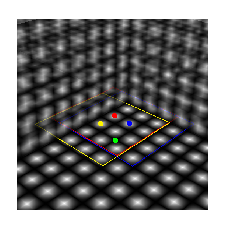
\epsfig{file = search_phase.eps, width = 6cm}}
  \caption{Different neighborhoods and their center pixel (red, yellow, blue) shown in a slice of the volume, one pixel (green) is affected by multiple neighborhoods}
  \label{fig:search_phase}
  \vspace{-0.1cm}
 \end{figure}
%
The sample image is divided into $9*9$ neighborhoods that overlap each other, these neighborhoods are vectorized \emph{i.e.} 
every texel from the neighborhood is stacked into a single vector. For RGB texels we have $9 * 9 * 3 = 243$ 
values in a single vector. It is possible to 
use a distance map as an extra channel by giving the algorithm a binary image as input, 
this is useful when the texture has large unstructured areas.
Once the vectors from the sample are constructed, we apply PCA 
(principal component analysis) \footnote{L. Smith 2002, A Tutorial on Principal Components Analysis; \url{www.cs.otago.ac.nz/cosc453/student_tutorials/principal_components.pdf}}
to reduce the dimensionality of each vector passing from $243$ to $18$ values approximately.
%
Reducing the vectors is a very convenient step, there are less values but we are still keeping $95\%$ of the relevant information.
The reduced vectors can be used to perform a standard closest neighborhood search in a high dimensional space. 
For this purpose, we use ANN library\footnote{ANN: A library for approximate nearest neighbor searching; \url{http://www.cs.umd.edu/~mount/ANN/} Mount, D. M. and Arya, S. 2006}.
%
\begin{equation}
 E(o, \{e\} ) = \sum_{t} \sum_{i \in \{x, y, z\}} \sum_{u \in N_i(t)} w_{t, i, u} ( o_{t, i, u} - e_{t, i, u} )^2
 \label{equ:imagenergy} 
\end{equation}
\begin{equation}
 w_{t,i} = || o_{t, i} - e_{t, i} ||^{r - 2}
 \label{equ:neighweight}
\end{equation}
%
During the search phase a weight for each neighborhood is calculated, for this purpose the energy function 
is written as equation \ref{equ:imagenergy} and the weight is calculated
as shown in equation \ref{equ:neighweight}. $N_i(t)$ represents the neighborhoods found in each dimension $x$, $y$, $z$ 
and $u$ is the texel in the neighborhood of $t$, this means that
a texel in the object is affected by multiple texels from different neighborhoods in the exemplar texture. 
The search is performed for every two texels $g_x = \{(i, 2 * j, 2 * k), \forall i, j, k \} $, $g_x$ 
is the voxel in a slice perpendicular to $x$. This is done similarly for $y$ and $z$, as shown in figure \ref{fig:search_phase}.
We set $r = 0.8$ to perform a robust optimization \cite{kwatra:2005:SIGGRAPH}.
%
Once the search phase is done the optimization phase takes place and it consists in averaging 
all the values found for each texel of the volume. 

\subsubsection{Optimization phase}
\label{sec:OptimizationPhase}
%
The optimization phase consists in averaging the values that affect one texel in the object. Note that
if the search phase is performed for every two texels as in \ref{sec:SearchPhase}, 
then the average will be for at most 75 texels (25 for each dimension).
%
\begin{equation}
 o_t = \frac{ \sum_{i \in \{x, y, z\}} \sum_{u \in N_i(t)} w_{u, i, t} * e_{u, i, t} }{ \sum_{i \in \{x, y, z\}} \sum_{u \in N_i(t)} w_{u, i, t} }
 \label{equ:texelaverage}
\end{equation}
%
Equation \ref{equ:texelaverage} shows the value of a texel in the object. 
When the texels present a high variability, the resulting object might be
blurred, in order to avoid this, 
clustering is performed to only average those texels that correspond to the principal cluster.
%
Following the optimization phase, the histogram matching is done to preserve the 
global statistics of the object relative to the exemplar.  

\subsubsection{Histogram Matching}
\label{sec:histogramMatching}
%
To perform histogram matching, the $CDF$ (cumulative distribution function) is calculated for both the exemplar and the object. 
Two $LUTs$ are constructed in order to perform faster calculations. The lookup table $LUT_o$ maps the grey level value of the object
to its corresponding value in the $CDF_o$, the lookup table $LUT_e$ maps the $CDF_e$
to the corresponding grey level value from the sample. 
The object is then modified by taking each of the texels $t$, using $LUT_o(t)$ to find the $CDF_o(t)$
and then using $LUT_e(CDF_o(t))$ to find the corresponding grey level value from the sample. The value of the object is then replaced 
by the corresponding value of the sample.

\section{\uppercase{Results and Evaluation}}
\label{sec:ResultsAndEvaluation}
We test our method to synthesize virtual MR images and virtual $SR \mu{CT}$images of trabecular bone (see Figure \ref{fig:ResultVolumes_exemplar}). 
The reference images were acquired for the needs of a study on osteoporosis, a disease inducing bone mass 
reduction and bone structure deterioration \cite{revol2002}. 
We have at our disposal a set of twelve 3D high resolution MR images with a cubic voxel of side 78$\mu$m and a set of twelve 3D 
$SR \mu{CT}$images downsampled to a resolution of 80$\mu$m to be on a comparable scale. As the MR images represent the marrow content of the samples, 
the contrast is inverted compared to $SR \mu{CT}$.
We generated 3D virtual SR$\mu$CT and $\mu$MR images (128x18x128 voxels) from two random reference slices (83x83 pixels) 
extracted from a volume taken out of the SR$\mu$CT and $\mu$MR sets (Figure \ref{fig:ResultVolumes_exemplar}).  
 
\begin{figure}
 \vspace{-0.2cm}
 \centering
 \subfigure[2D reference textures extracted from real images and binary masks.]{
 			\label{fig:ResultVolumes_exemplar}
%	    
\epsfig{file = 42.irm_Y_015.eps, width = 1cm}
%	    
\epsfig{file = 42.irm_Y_015Mask.eps, width = 0.5cm}            
%	    
\epsfig{file = 42.irm_Y_047.eps, width = 1cm}
%	    
\epsfig{file = 42.irm_Y_047Mask.eps, width = 0.5cm}
%	    \hspace{0.5cm}
%	    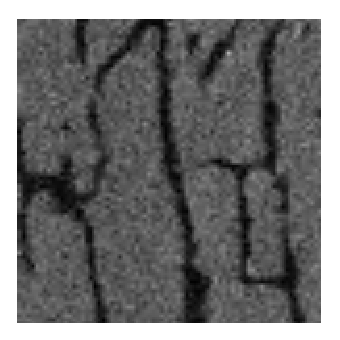
\epsfig{file = vol.73-93-94-sliceX.eps, width = 1cm}
%	    
\epsfig{file = vol.73-93-94-sliceXMask.eps, width = 0.5cm}                        
%	    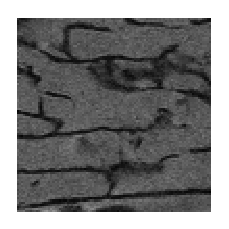
\epsfig{file = vol.73-93-94-sliceZ.eps, width = 1cm} 
%	    
\epsfig{file = vol.73-93-94-sliceZMask.eps, width = 0.5cm}}\\
% \subfigure[3D virtual images.]{
% 			\label{fig:ResultVolumes_textures}
% 			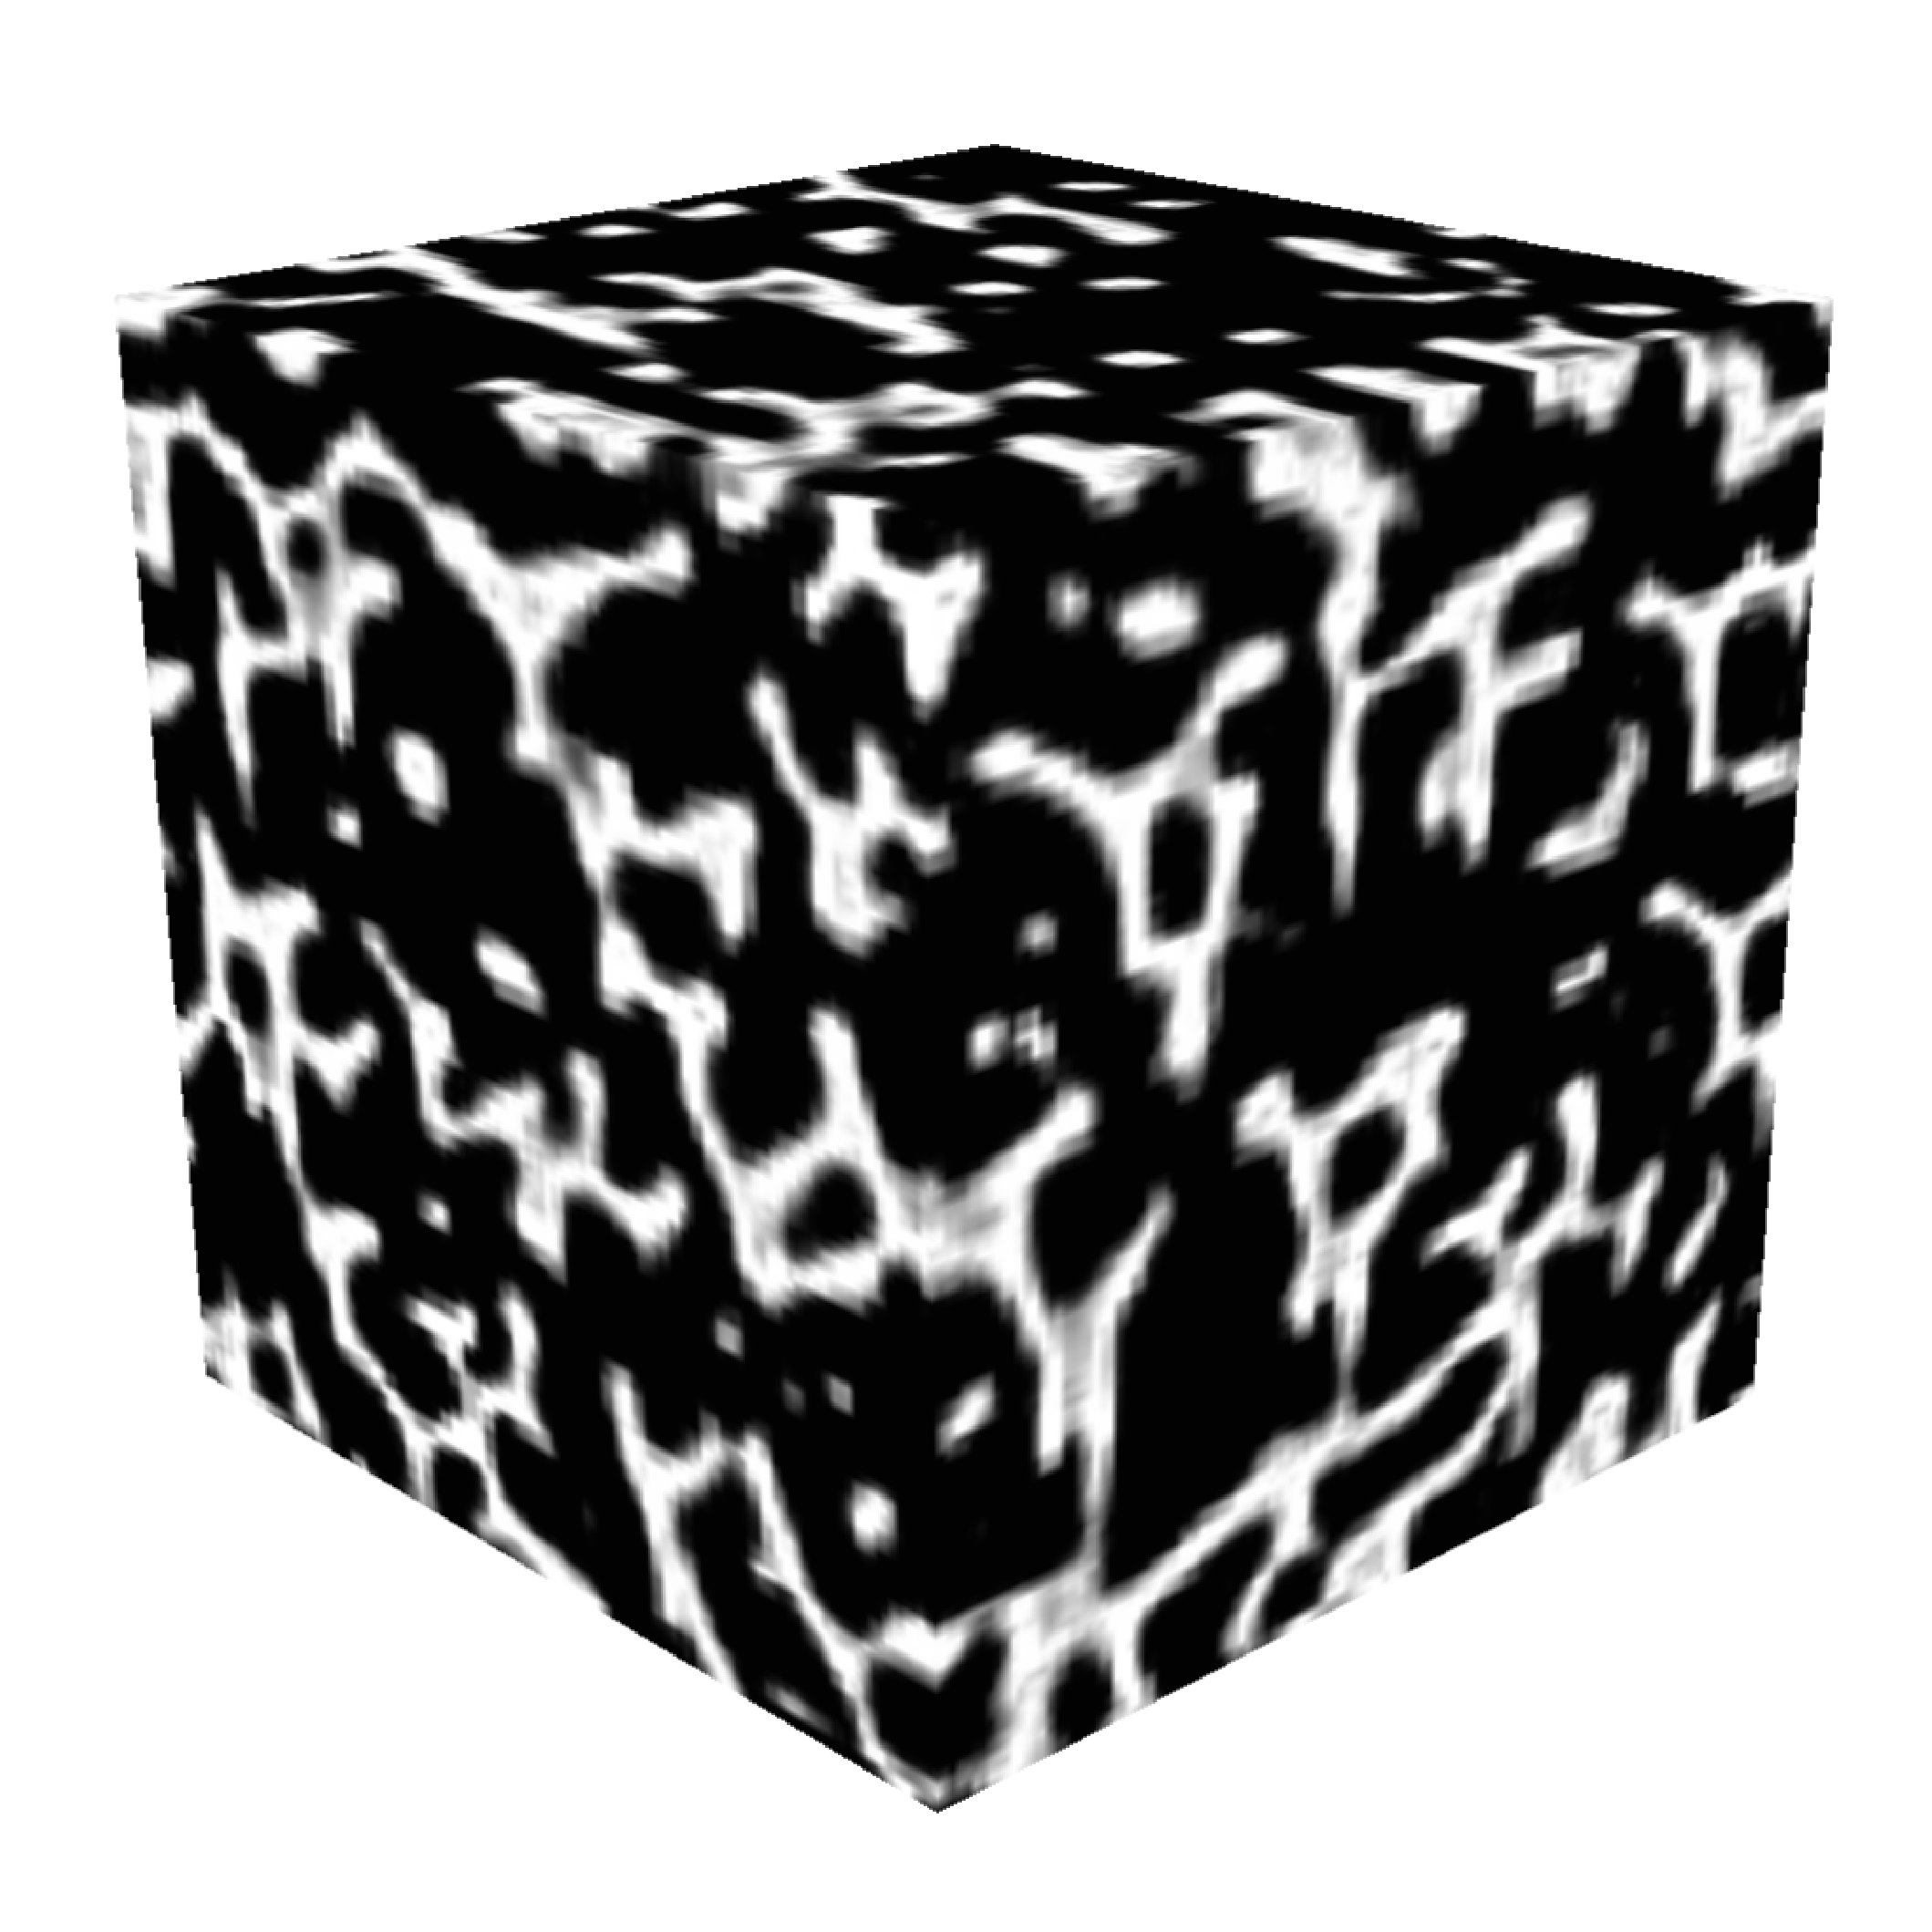
\epsfig{file = ModelESRF.eps, width = 3cm}
%			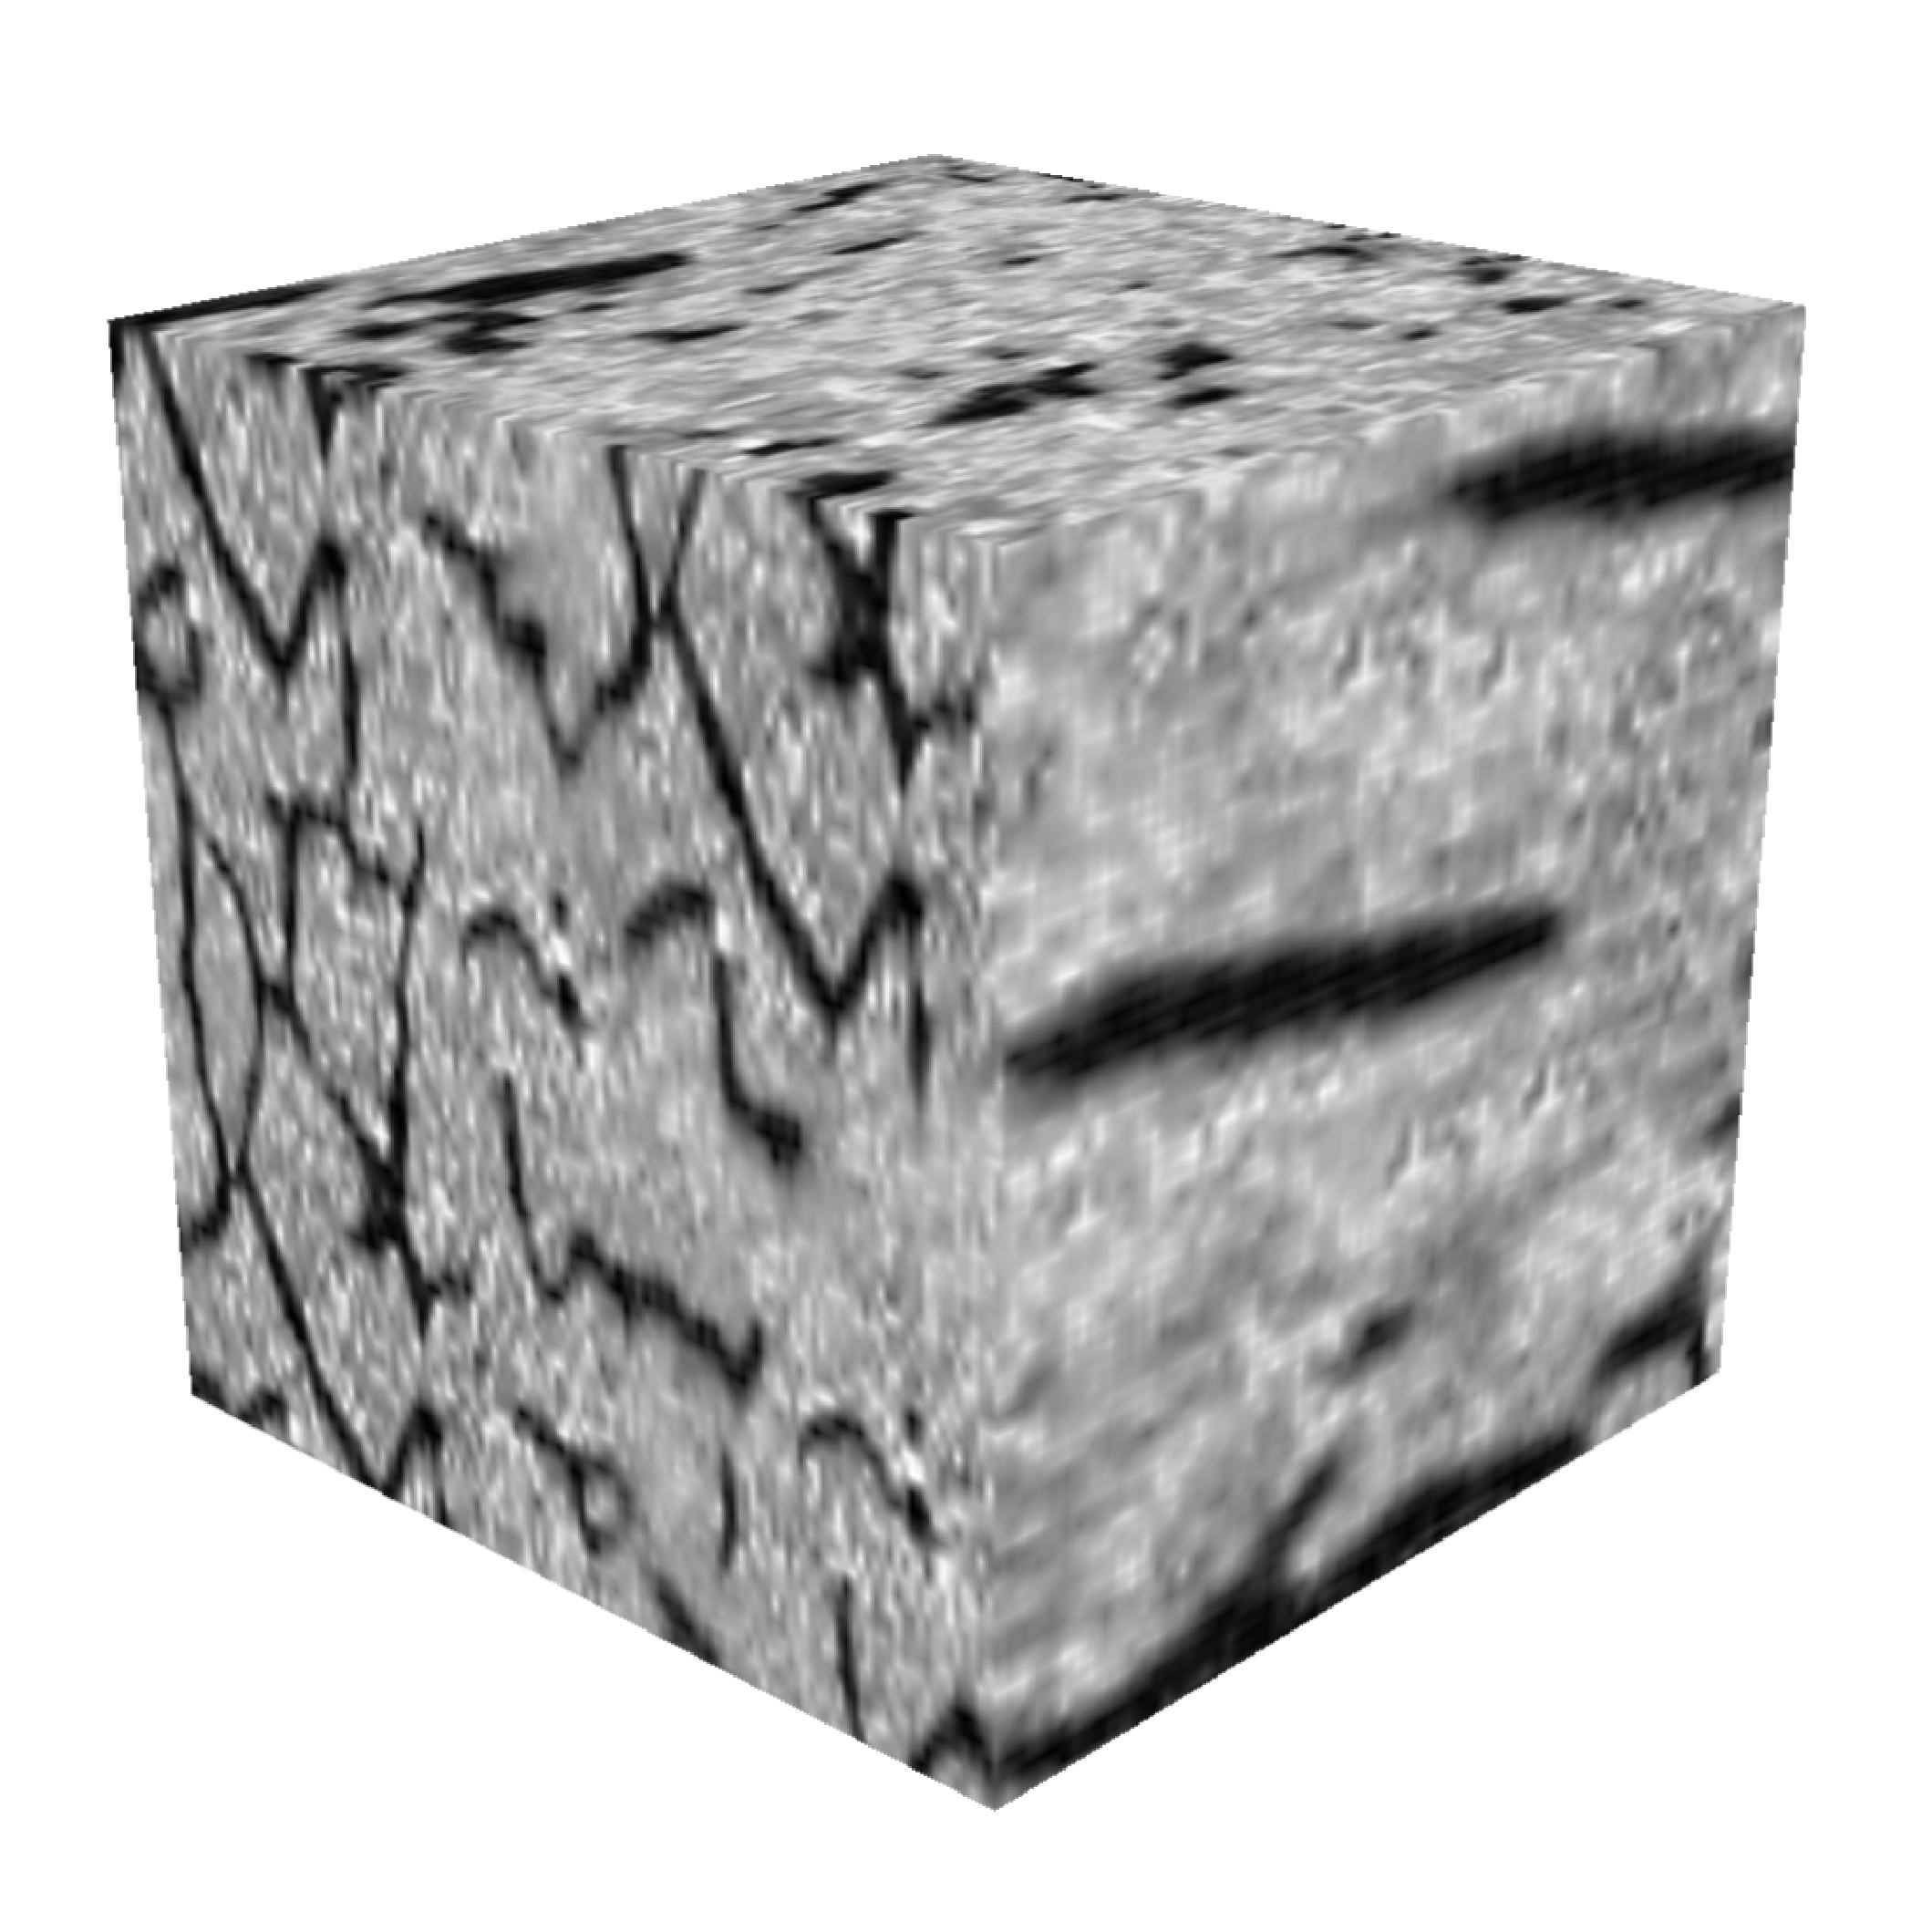
\epsfig{file = ModelIRM.eps, width = 3cm}
      
\epsfig{file = 42.irm_Y_015.eps, width = 1.20cm}
	    
\epsfig{file = 42.irm_Y_015Mask.eps, width = 0.70cm}            
	    
\epsfig{file = 42.irm_Y_047.eps, width = 1.20cm}
	    
\epsfig{file = 42.irm_Y_047Mask.eps, width = 0.70cm}
	    \hspace{0.20cm}
	    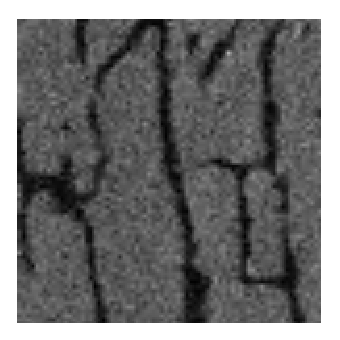
\epsfig{file = vol.73-93-94-sliceX.eps, width = 1.20cm}
	    
\epsfig{file = vol.73-93-94-sliceXMask.eps, width = 0.70cm}                        
	    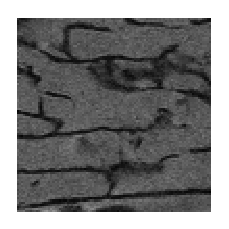
\epsfig{file = vol.73-93-94-sliceZ.eps, width = 1.20cm} 
	    
\epsfig{file = vol.73-93-94-sliceZMask.eps, width = 0.70cm}}\\
 \subfigure[3D virtual images.]{
 			\label{fig:ResultVolumes_textures}
 			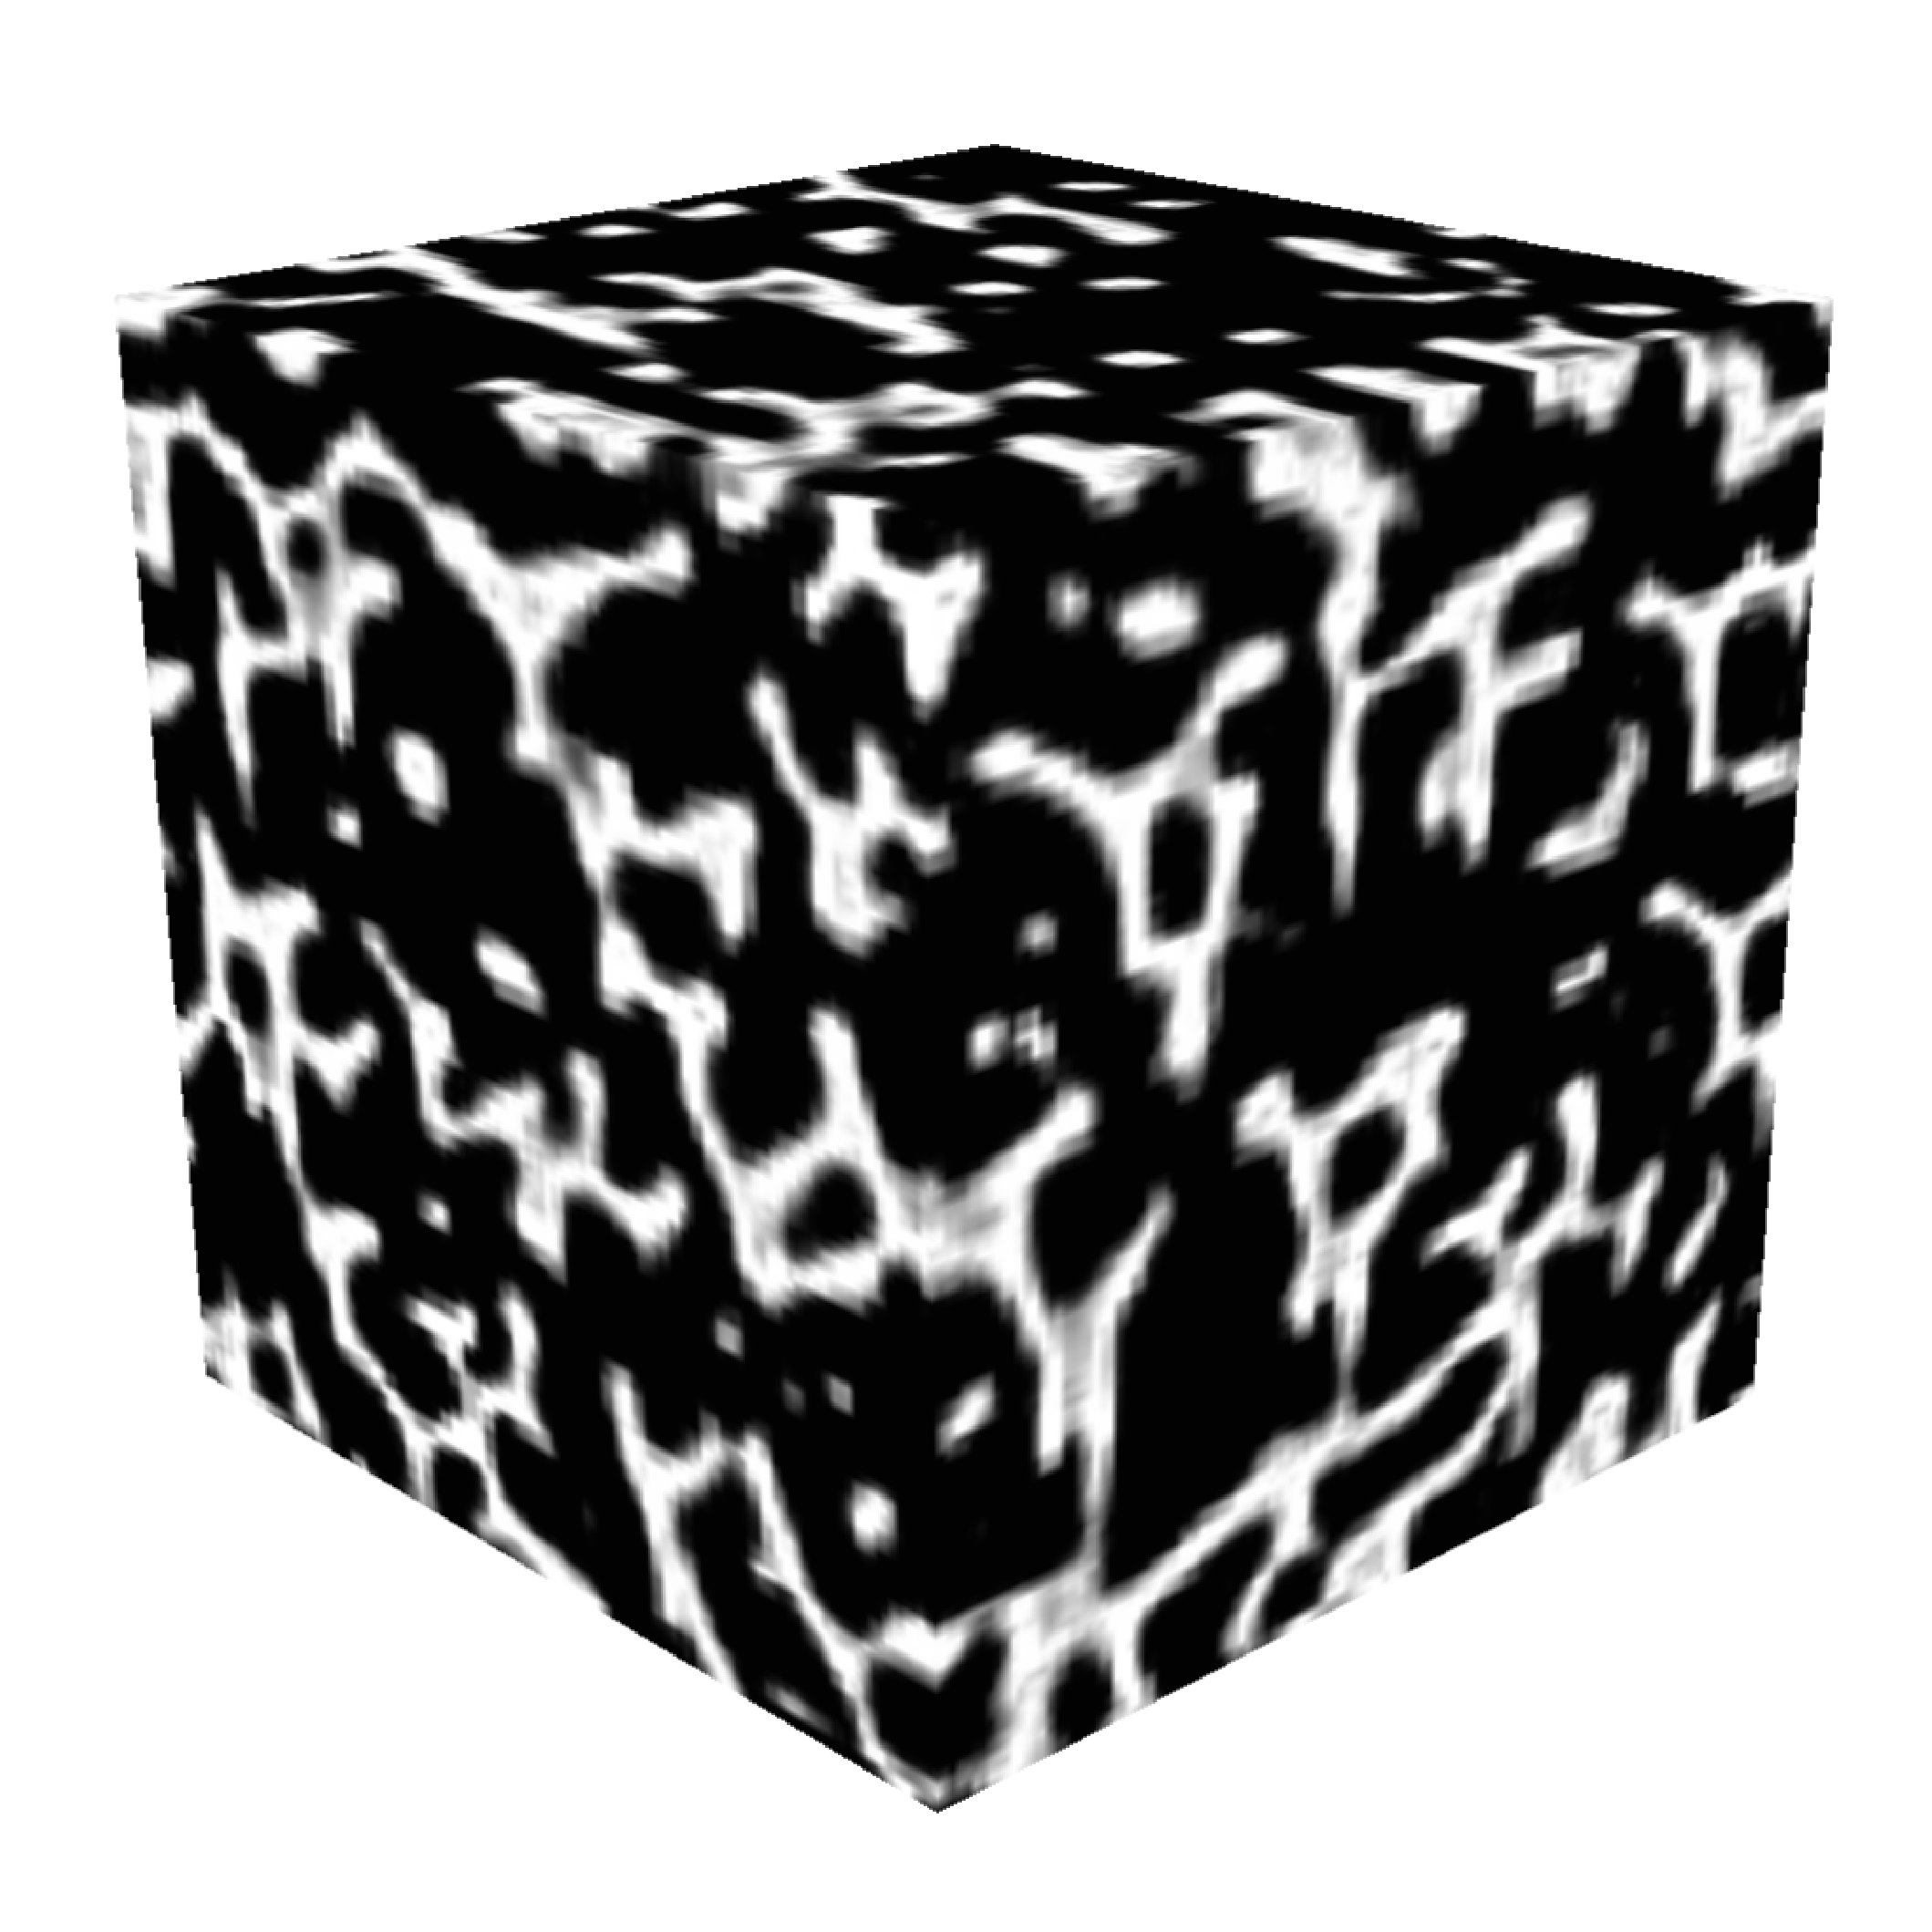
\epsfig{file = ModelESRF.eps, width = 4.5cm}
			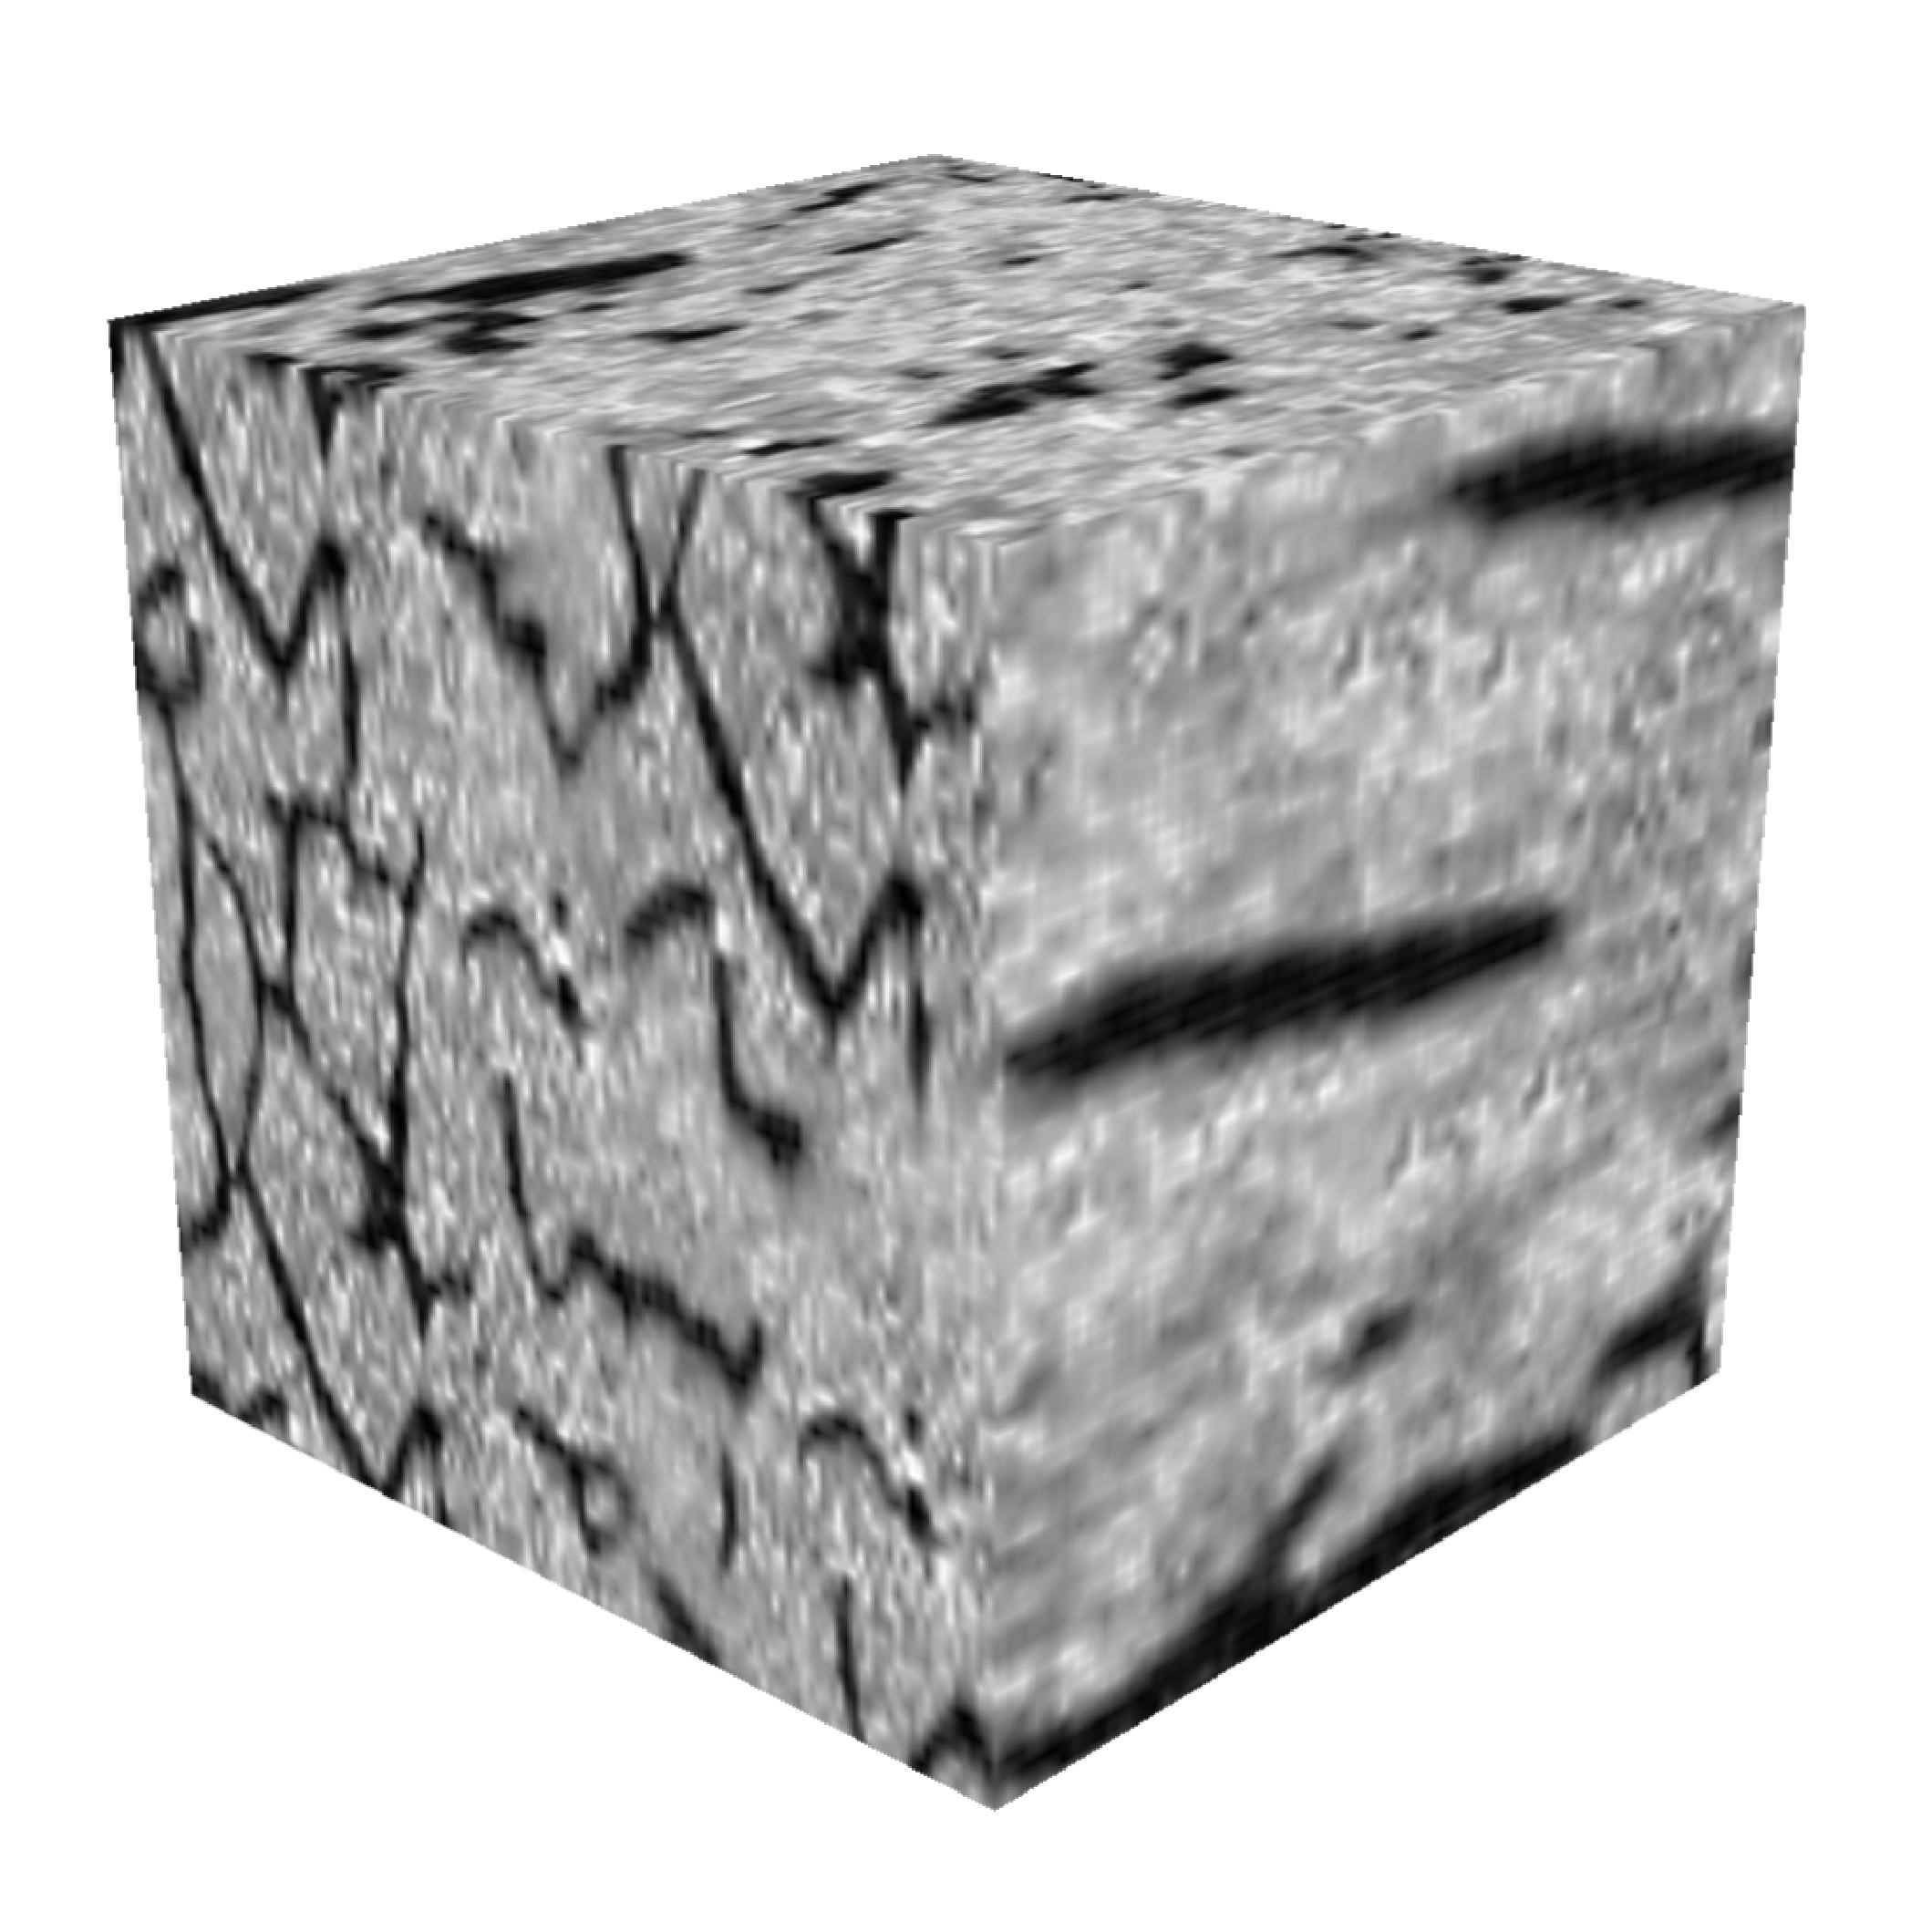
\epsfig{file = ModelIRM.eps, width = 4.5cm}
			      } 
 \caption{Results of synthesis for $SR \mu{CT}$ (left) and $\mu{MRI}$ (right) using multiple textures to constrain plans perpendicular to axis-directions and binary masks to enhance the untextured areas.
         }
 \label{fig:ResultVolumes}
 \vspace{-0.1cm}
\end{figure}

We assess the accuracy of the virtual images from a statistical and a morphological point of view. As the ultimate goal is to produce synthetic images as close as possible 
to the reference ones, we compare their grey level distributions and some morphological bone parameters computed from their content. 
In this study, we only evaluate the quality of virtual $\mu$MR images.%(3D texture generated from SR$\mu$CT images has already been validated in  \cite{prieto2012}).


\subsection{\uppercase{Statistical assessment }}
\label{sec:Statistics}
%
Figure \ref{fig:histograms} shows the histograms of the exemplar texture and the synthetic 3D $\mu{MR}$ 
image shown in Figure \ref{fig:ResultVolumes}. 
Note that when a randomly chosen slice is taken from the synthetic volume, the values of the histogram will be close to those of the exemplar,
therefore, global statistics are still preserved. 
Thanks to the histogram matching, 
the grey levels distribution of the marrow and the bone are quite similar in the virtual image and the reference image. 
The statistics displayed near each histogram (mean, standard deviation, mode) are also very close.
%
\begin{figure}
 \centering 
 \subfigure[2D sample]{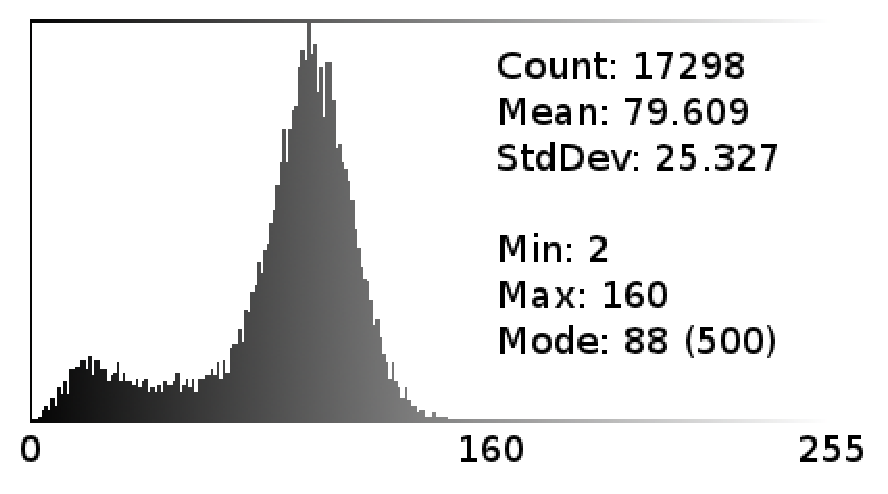
\epsfig{file = HistoSampleIRM.eps, width = 4cm}}
 \subfigure[3D synthetic image]{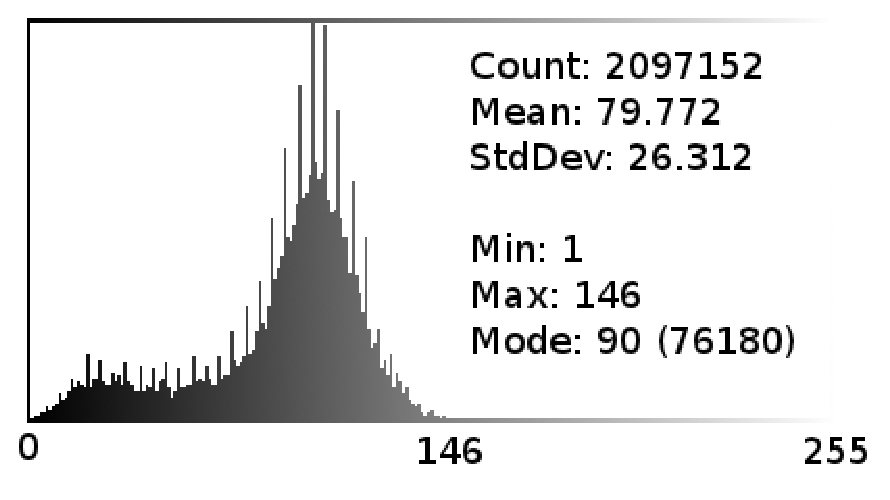
\epsfig{file = HistoModelIRM.eps, width = 4cm}}
\caption{Comparison of the histograms obtained from the reference 2D and the 3D synthetic $\mu{MR}$ image.}
 \label{fig:histograms}
\end{figure}

\subsection{\uppercase{Morphological assessment}}
\label{sec:Morphology}
\noindent
In this part, we quantitatively compare some structural parameters of bone architecture obtained from the real and the synthetized $\mu$MR images.
As displayed in Figure \ref{fig:histograms}, the bone and marrow distribution are clearly overlapping, thus making the segmentation difficult. A more sophisticated method than a simple thresholding must be used to extract the trabecular bone. The same segmentation method was applied on the real and the virtual images \cite{PR2002}. This step is essential for the computation of the bone parameters.  %We propose to quantitatively assess the accuracy of the morphological structure given by our synthetic 3D texture. 
%For this study, we generate a 3D texture from SR$\mu$CT images provided a few years ago by 
%the European Synchrotron Radiation Facility (ESRF) in Grenoble for the needs of a study focused on osteoporosis. 
%Osteoporosis is a bone fragility disease leading to spontaneous bone fractures and characterized by a bone mass reduction and a bone structure deterioration. 
%The images present a high resolution level
%with an isotropic voxel of 10 $\mu$m width and a volume size of 330x330x330 pixels helpful to assess trabecular bone architecture \cite{revol2002}. 

%
We computed 3D morphological and topological architecture parameters from a set of twelve real $\mu$MR images and from a set of ten virtual $\mu$MR images. 
A 3D MIL (Mean Intercept Length) method was chosen to produce parameters related to the trabecular bone morphology and the Euler number was computed to estimate the bone topology. 
We considered the seven following parameters: Partial Bone Volume (BV/TV), Bone Surface to Bone Volume ratio (BS/BV), Trabecular Thickness (Tb. Th), Trabecular Number (Tb. N), Trabecular Separation (Tb. Sp)and Mean Intercept Length (MIL1). 
The connectivity was estimated by the Euler number (Euler/mm3)normalized by the total volume. The higher the Euler number's value, the less connected the bone structure is.

\begin{figure}
 \centering 
 \subfigure{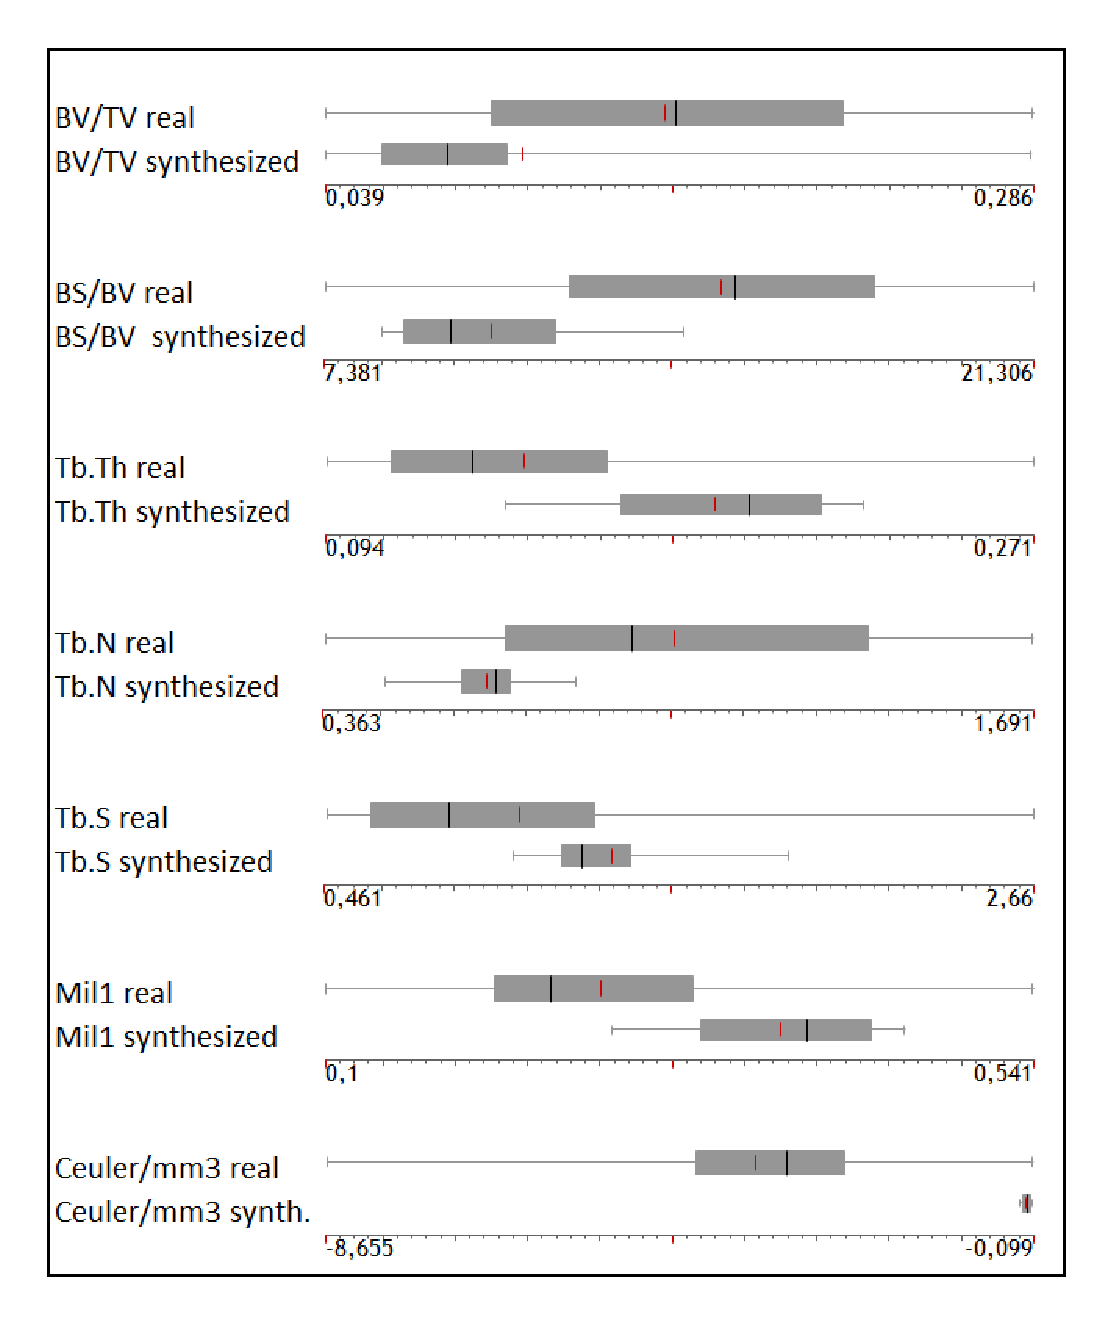
\epsfig{file = boxplots.eps, width = 8cm}} 
\caption{Boxplots of morphological and topological bone parameters computed from real and synthetic $\mu$MR images.}
 \label{fig:bone_parametres}
\end{figure}

We assess the accuracy of the virtual images by comparing the bone parameters computed from the set of 
$\mu$MR images with those computed from synthetic ones. Figure \ref{fig:bone_parametres} displays the boxplots associated to each bone parameter obtained from the sets of real and virtual $\mu$MR images. For the chosen representation, whiskers ends at minimum and maximum values, box starts at Q1 (first quartile) and ends at Q3 (third quartile), median appears in black, average in red. The scale line above the boxplots show the range of values of each parameter. It can be noticed that for all the morphologic parameters the distributions of the parameters computed from the virtual images are included in the range of values of those computed from the real images, thus proving the resemblance of the virtual bone with the real bone. They are also less spread, so the variability of the generated bone structures is reduced compared to the real set. Another set of randomly chosen reference slices would yield different results. 
For the topologic parameter (Euler/mm3), the score is slightly higher than the maximum value obtained with the $\mu$MR set, which remains satisfying. It means that the bone structure in the virtual images has a somewhat lower connectivity than in the reference set.  

\begin{figure*}
 \vspace{-0.2cm}
 \centering 
\subfigure[Synthetic volume.]{
			      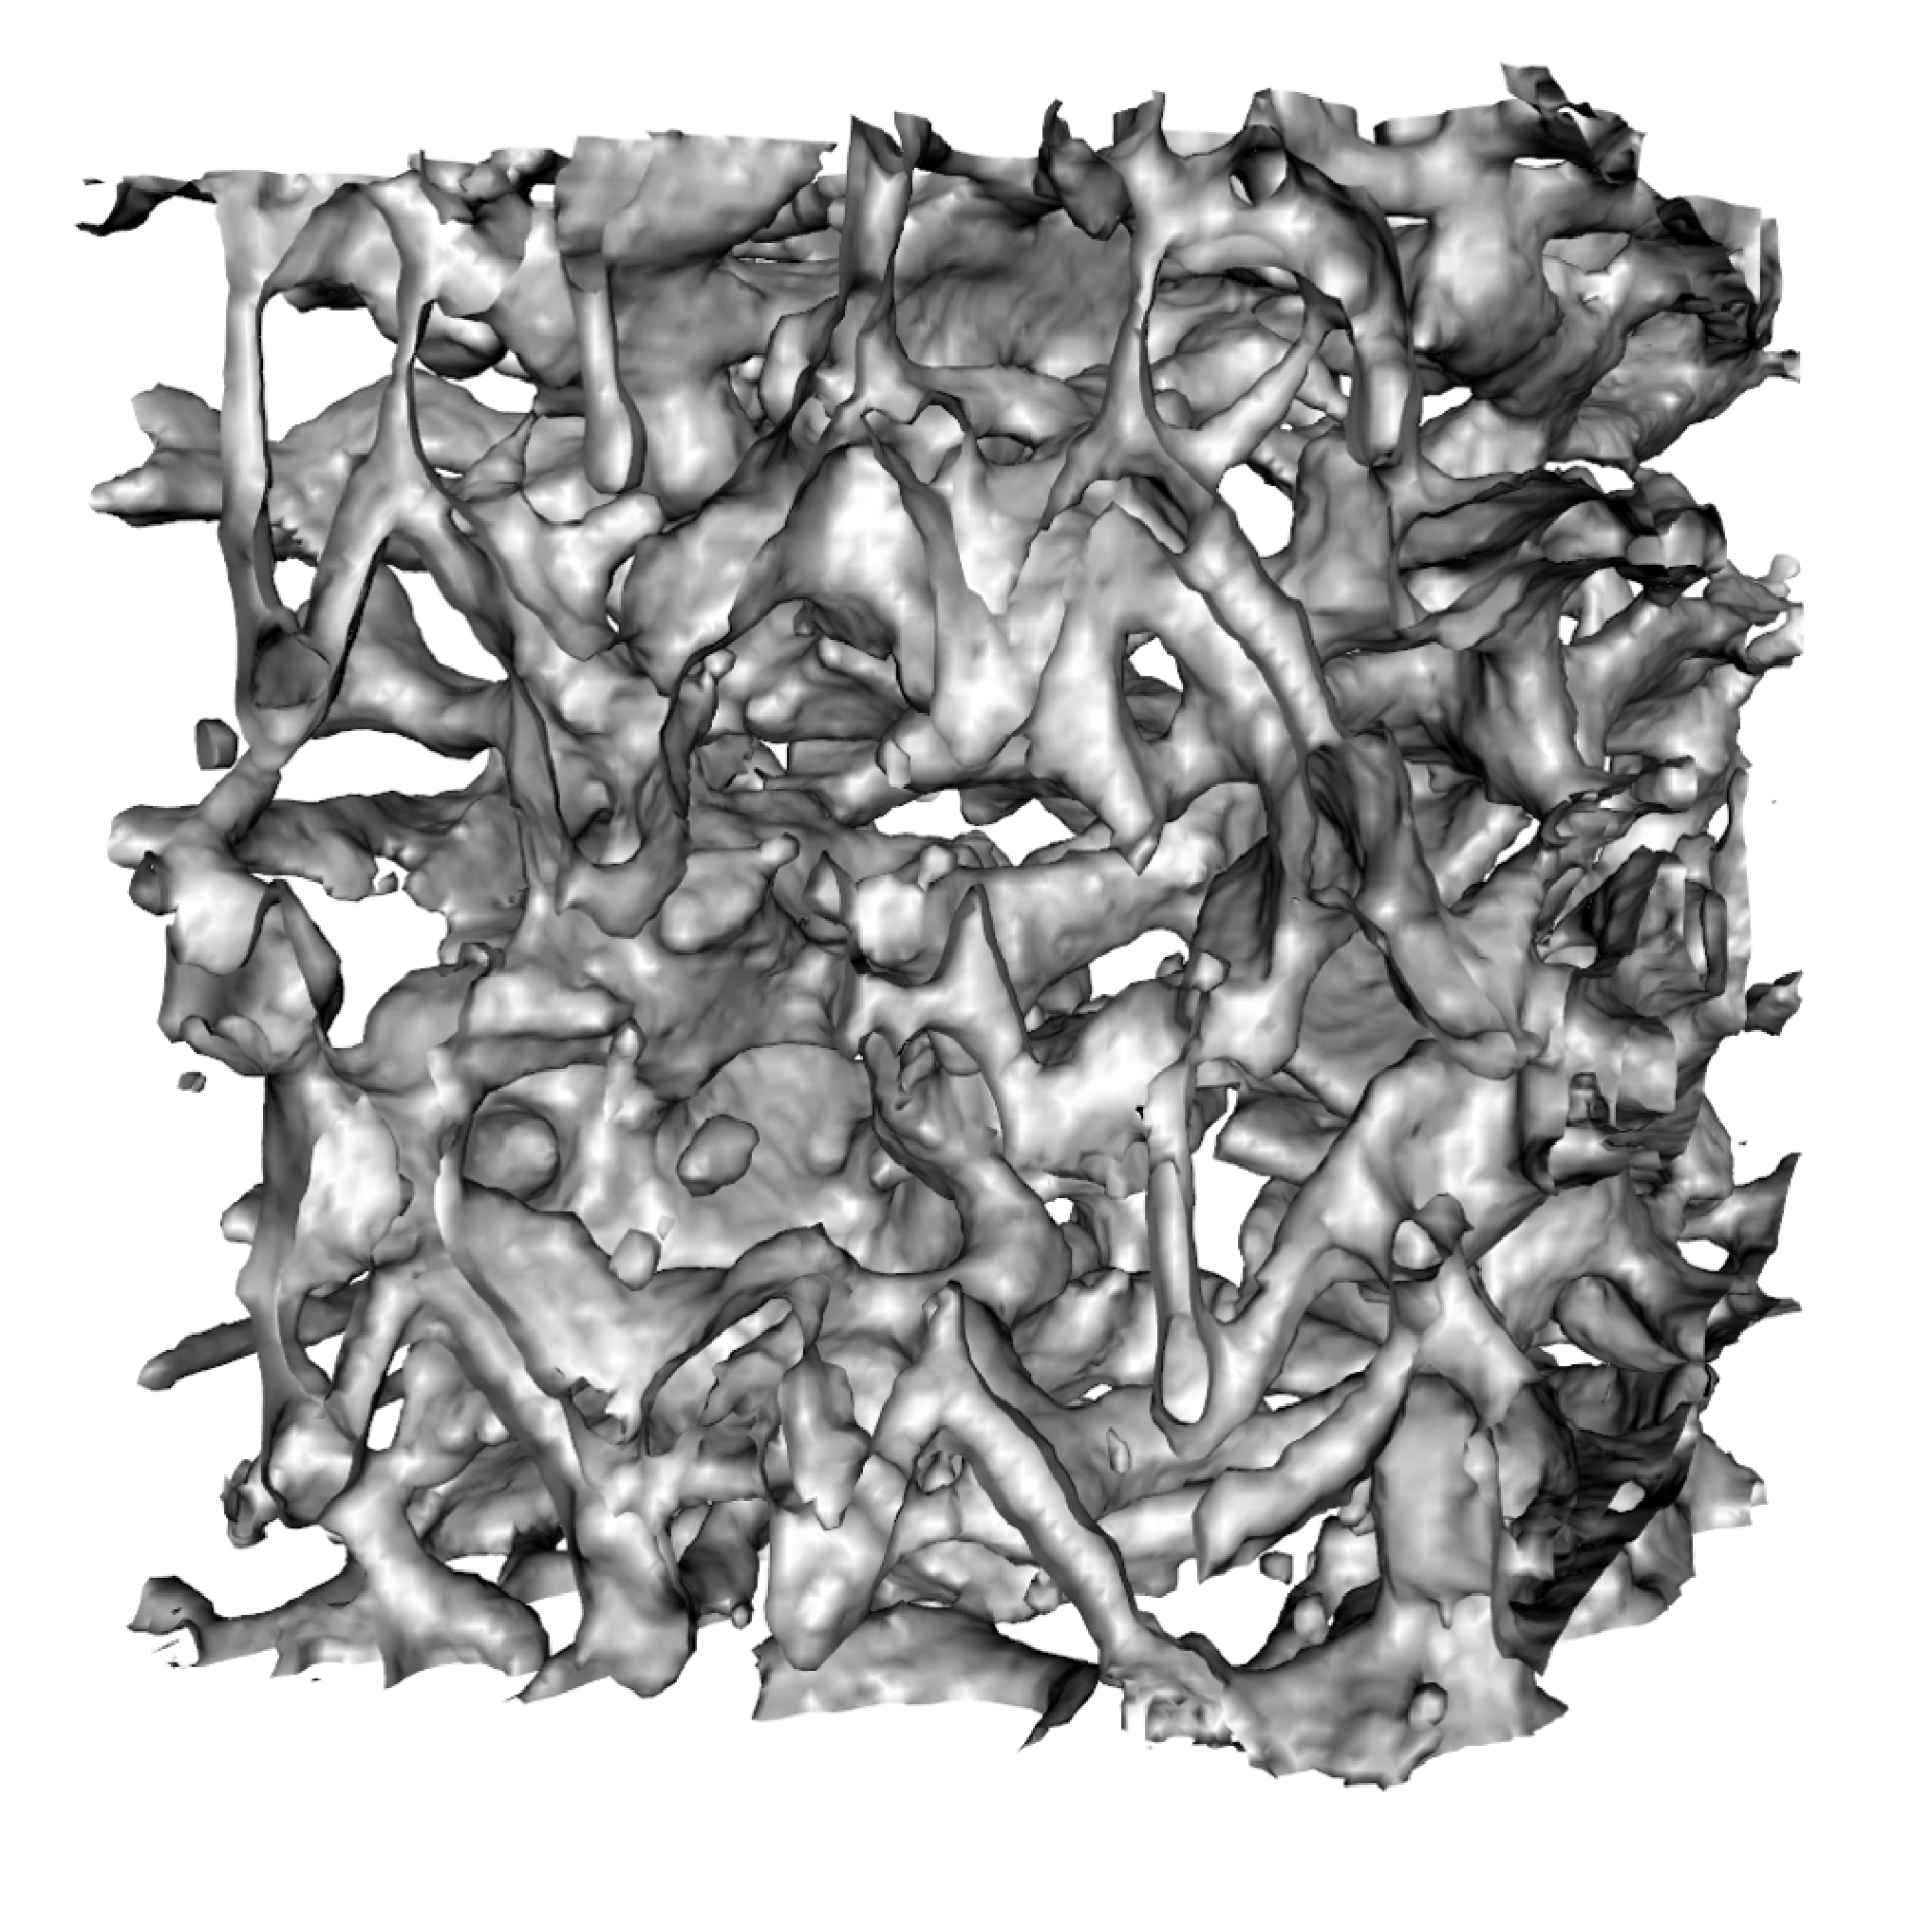
\epsfig{file = synthetic0.eps, width = 6.5cm}
			      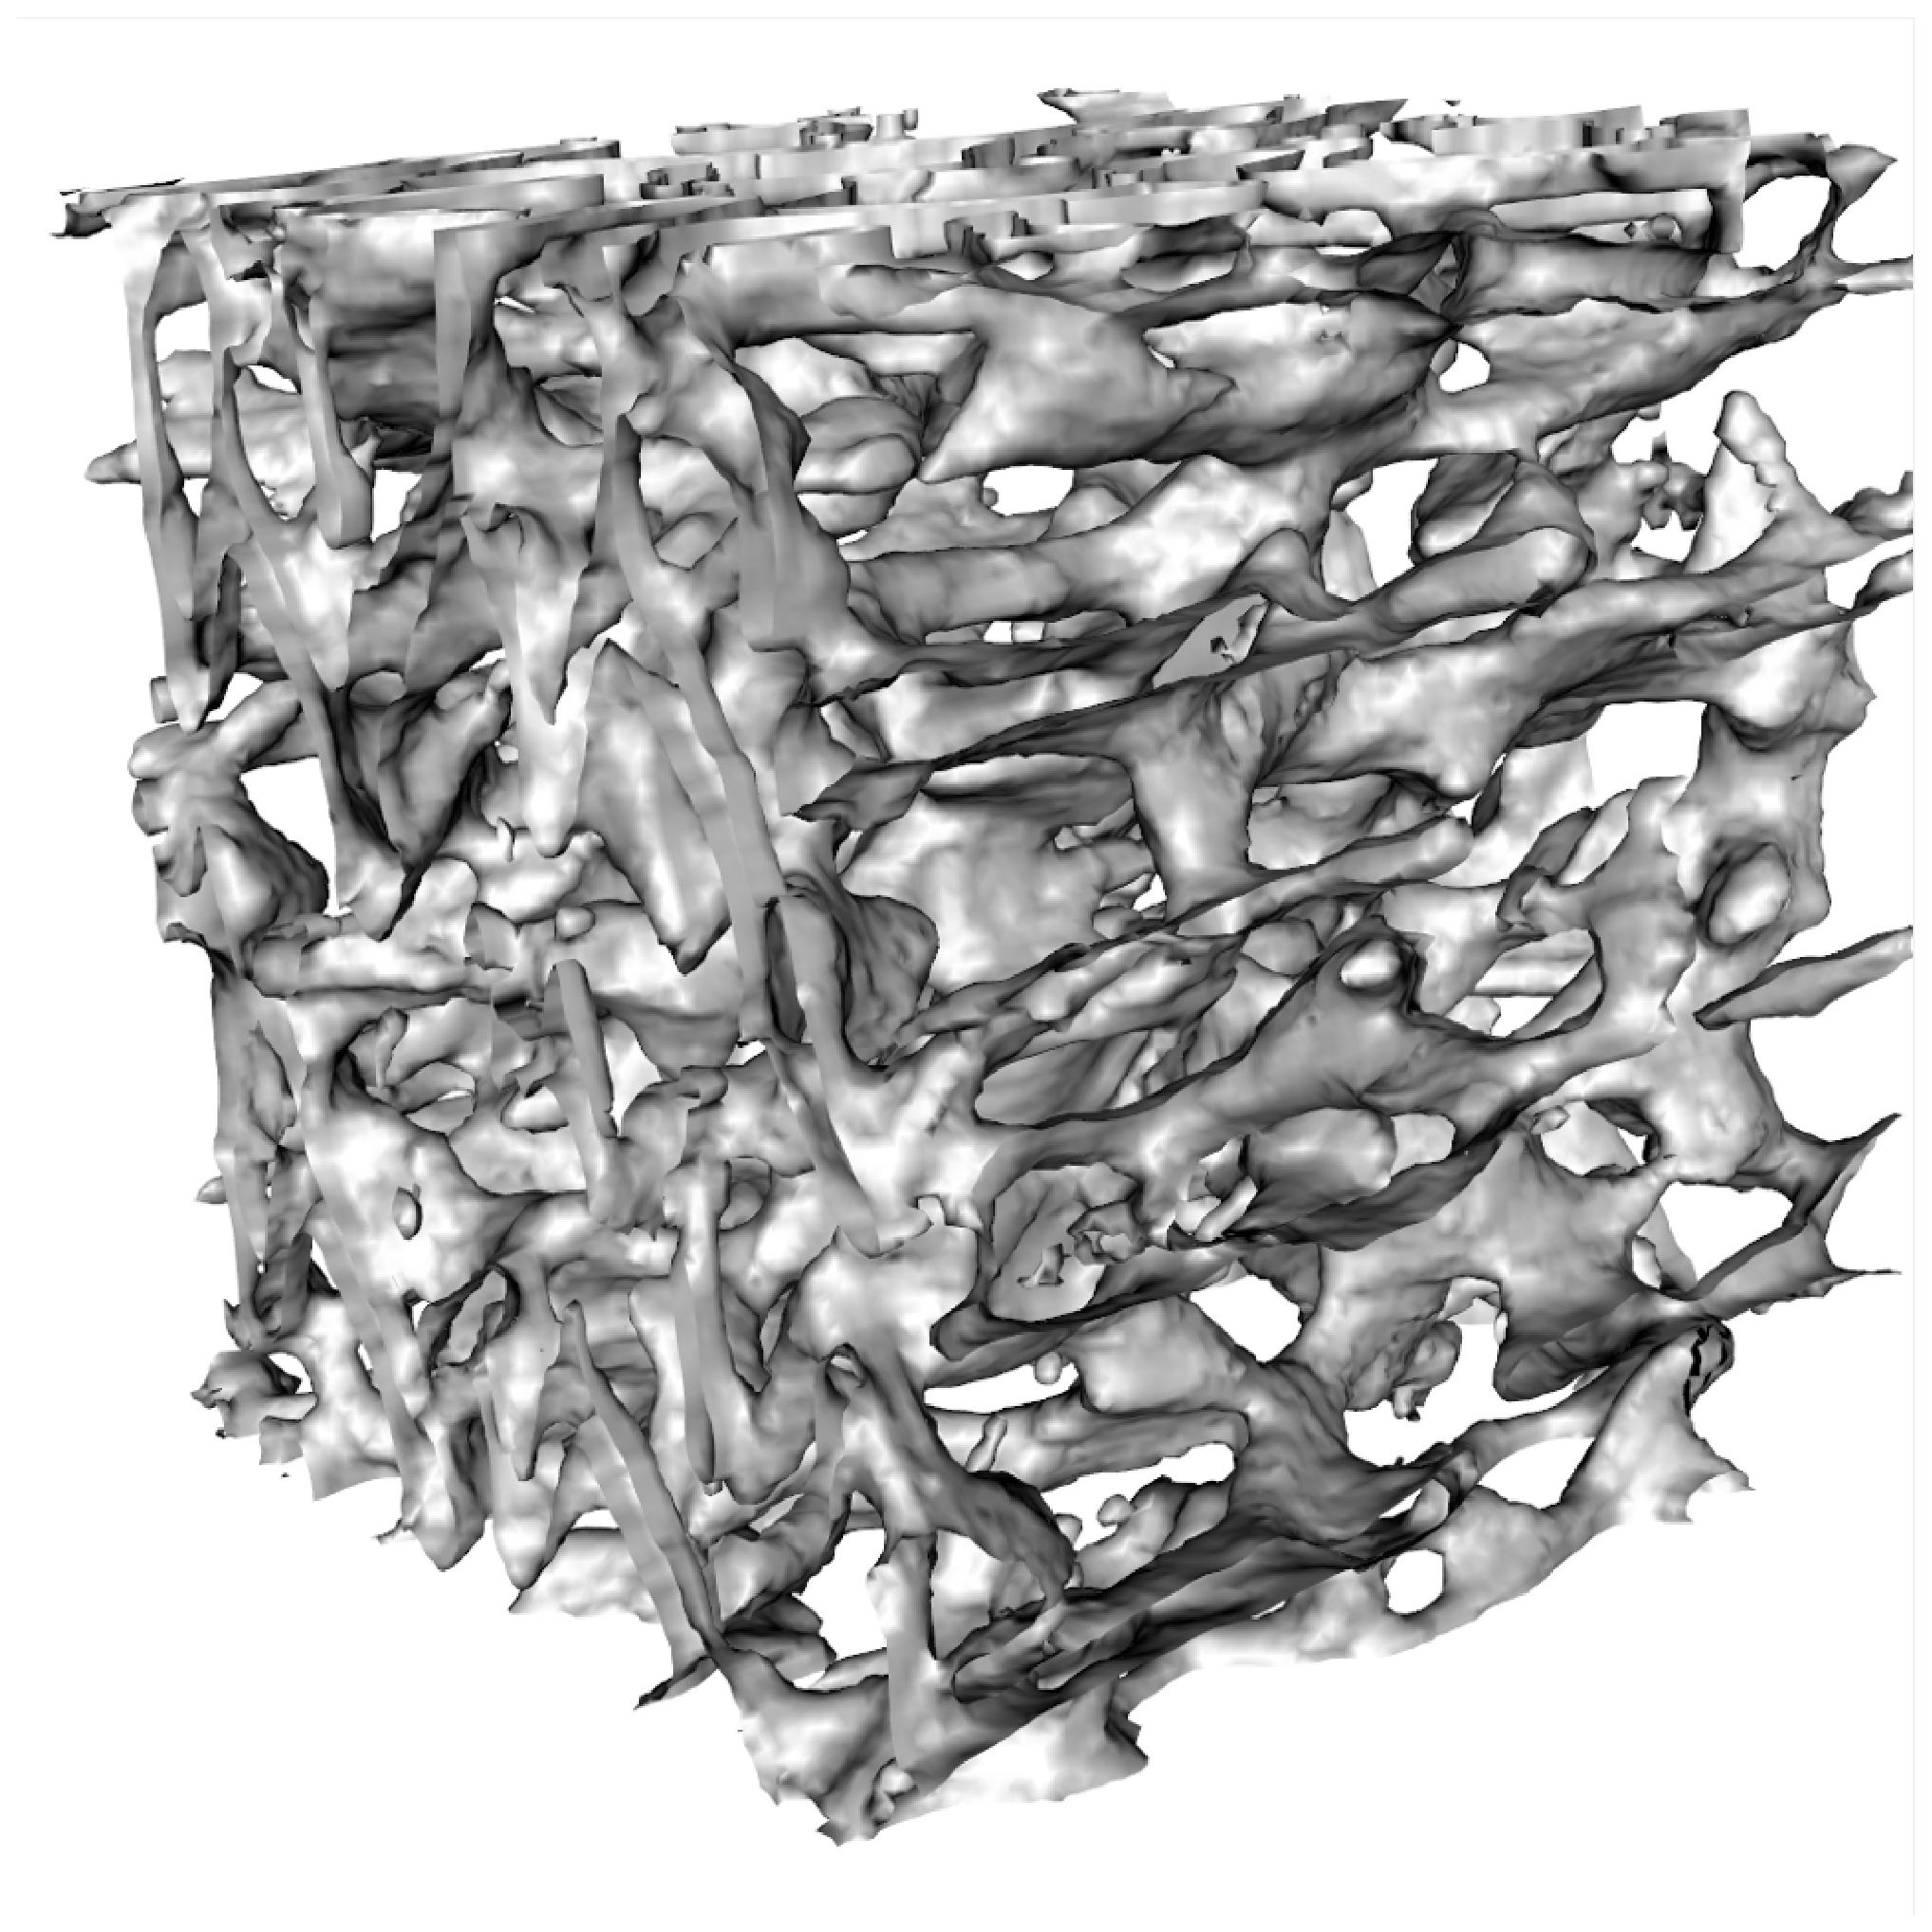
\epsfig{file = synthetic1.eps, width = 6.5cm}
			     }
\subfigure[Original volume.]{
			      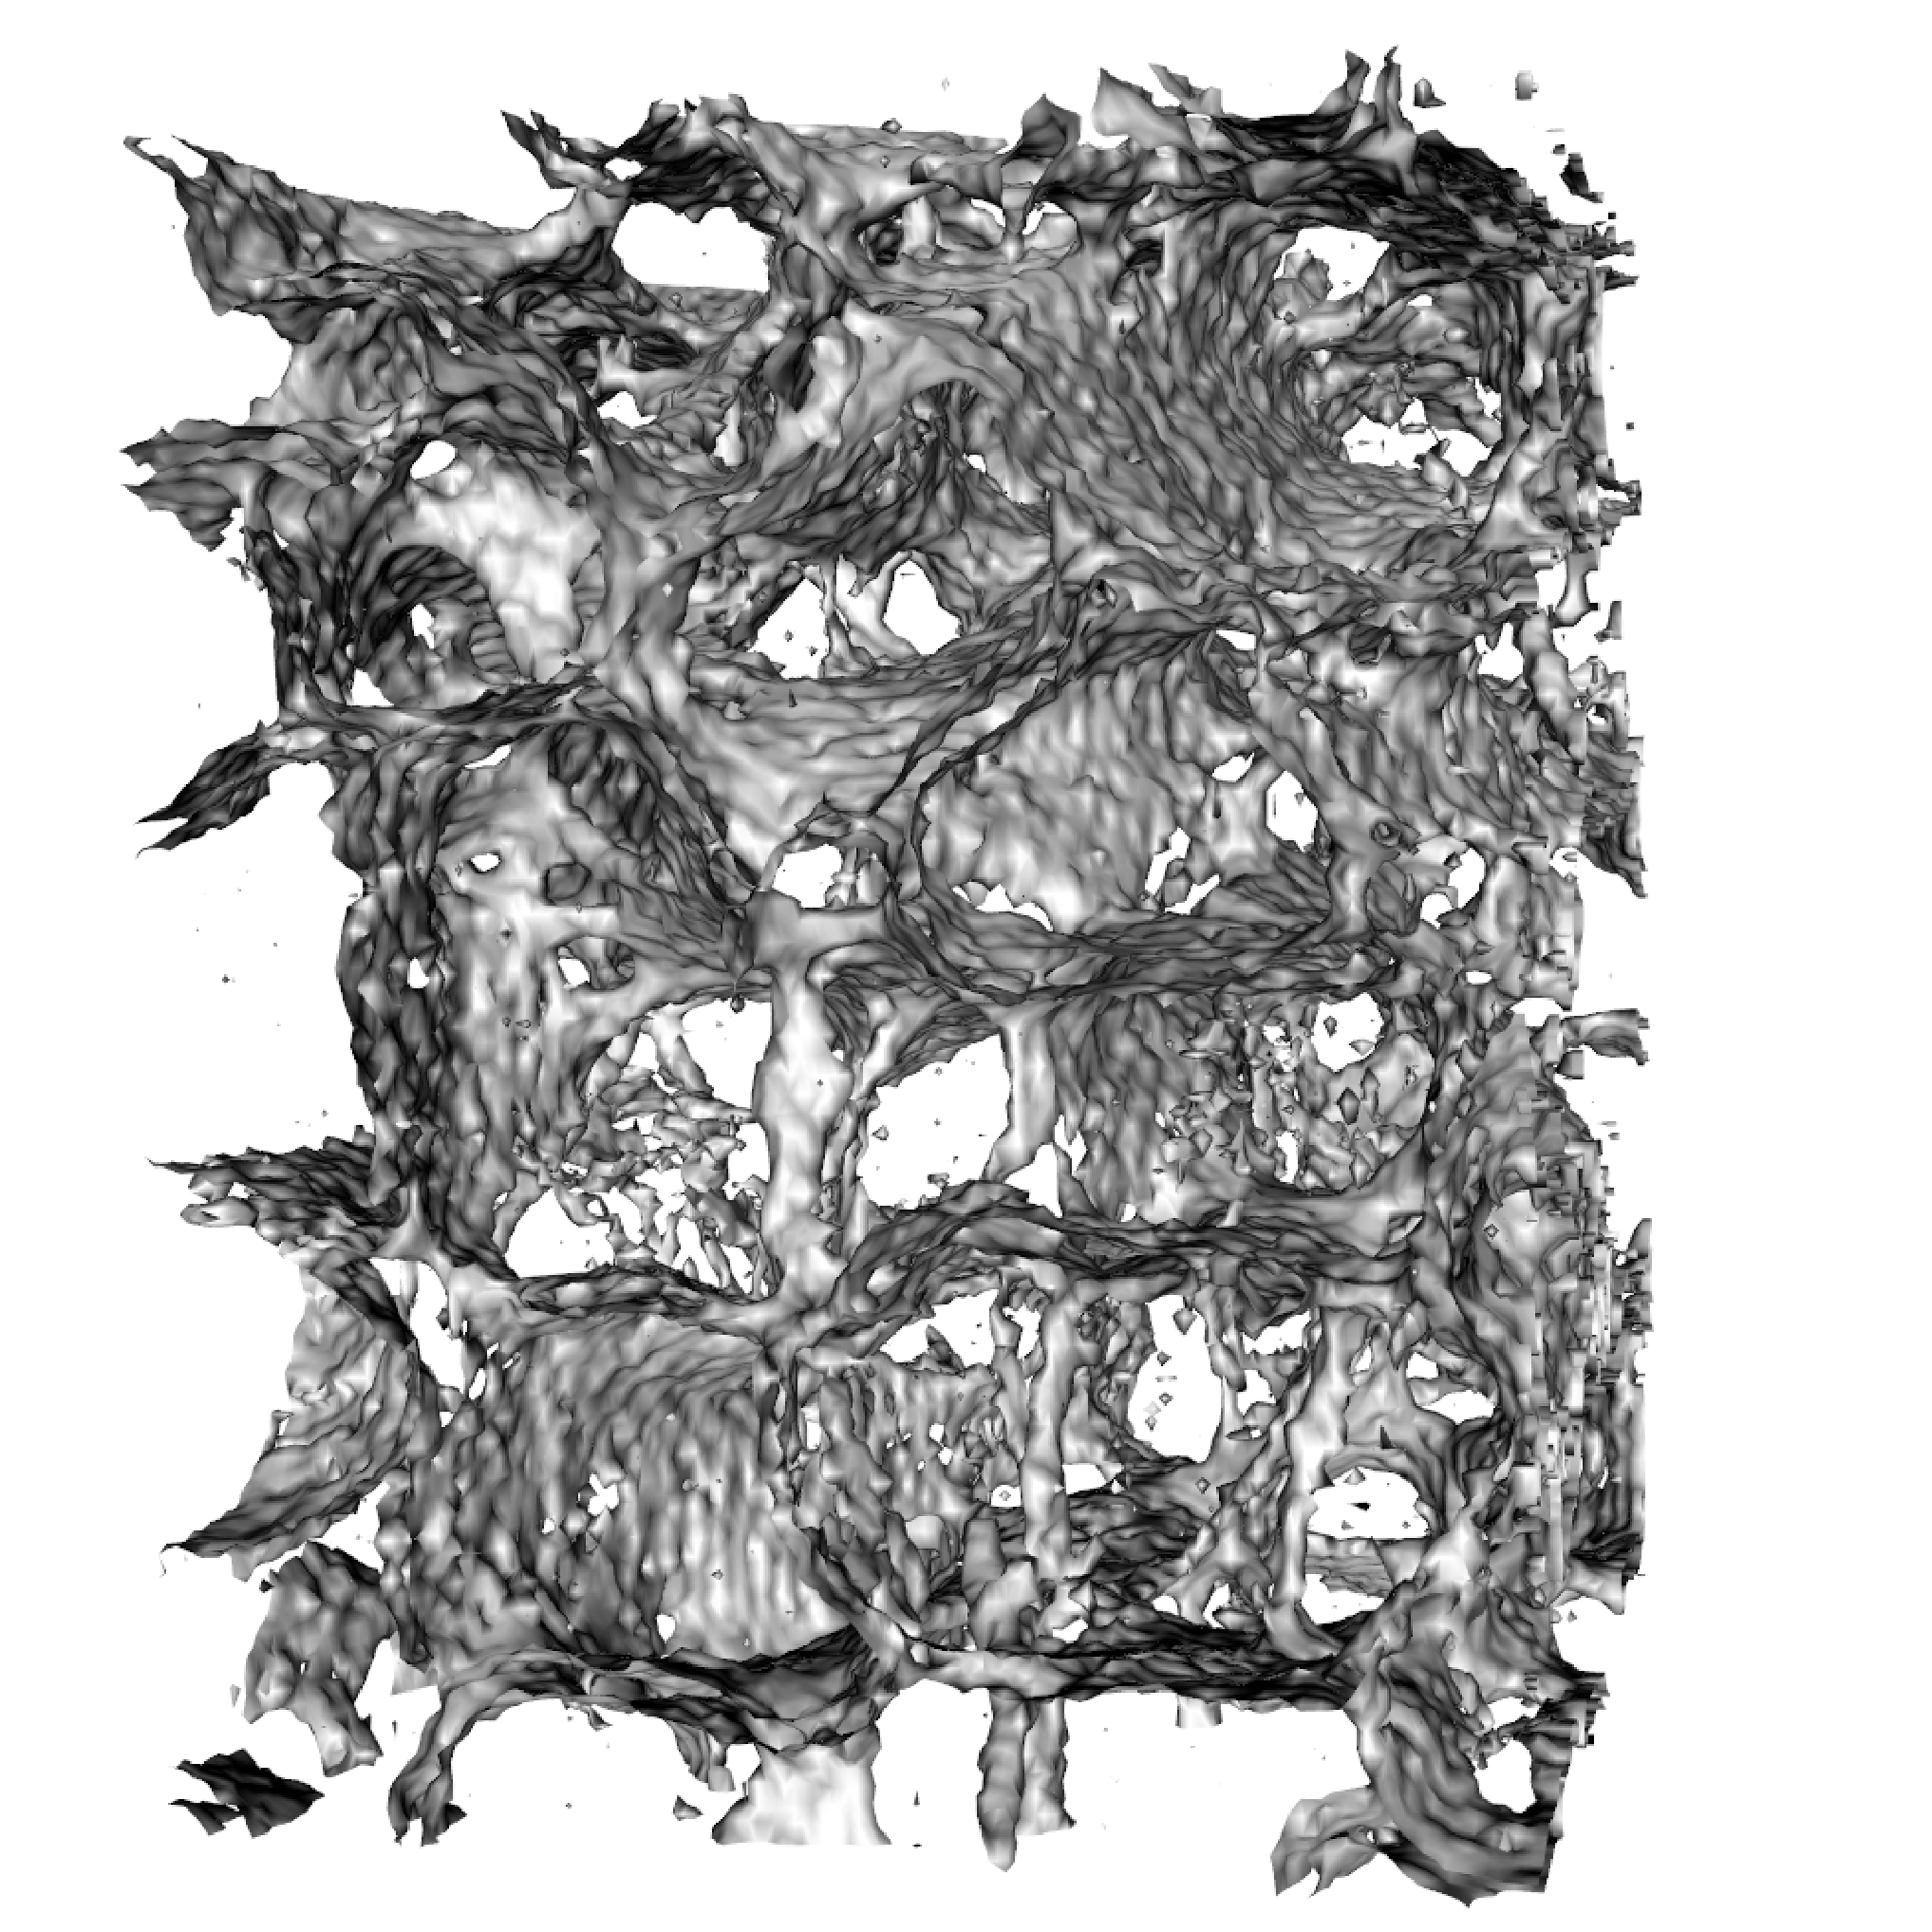
\epsfig{file = original0.eps, width = 6.5cm}
			      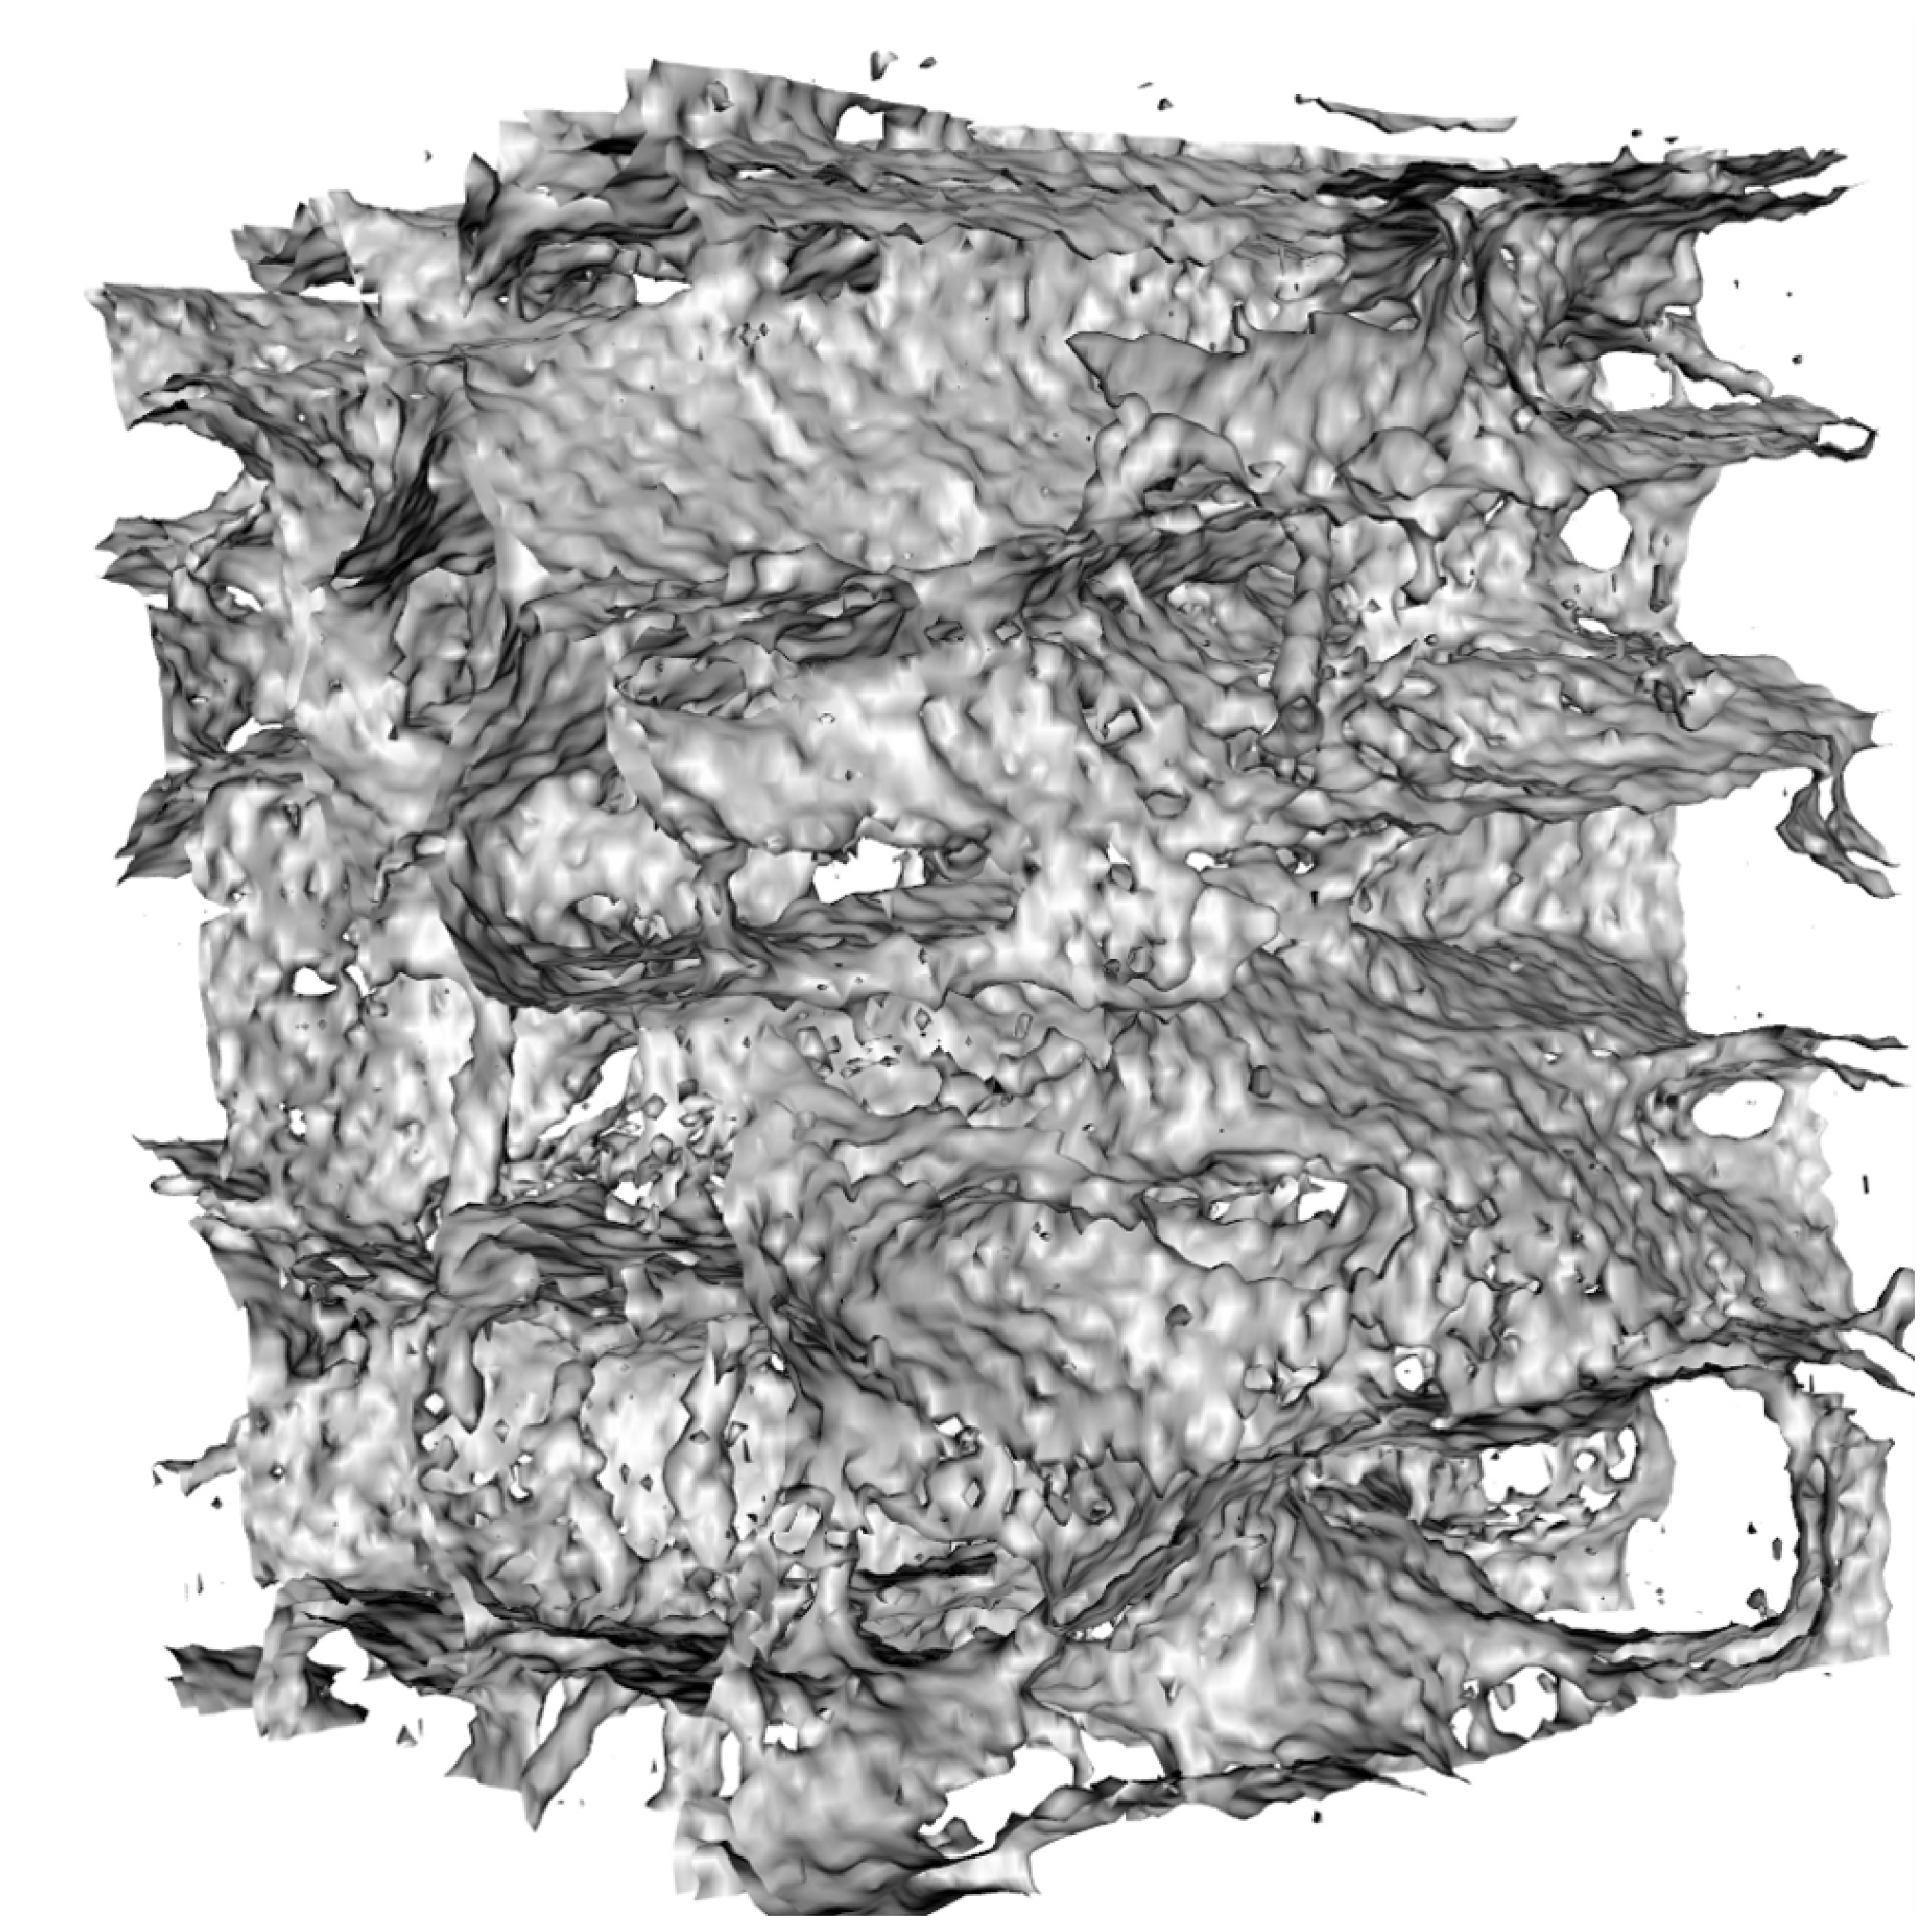
\epsfig{file = original1.eps, width = 6.5cm}
			    }
 \caption{Surface rendering of trabecular bone architecture obtained with: a) virtual $\mu$MR image, b) real $\mu$MR image.}
 \label{fig:bone_surface_rendering}
 \vspace{-0.1cm}
\end{figure*}
%
In Figure \ref{fig:bone_surface_rendering}, segmented trabecular bones from the 3D virtual $\mu$MR images are compared to those obtained from the 3D $\mu$MR image 
from which were taken the reference slices for the texture synthesis. We retrieve visually the similarity demonstrated by the bone parameters.

\section{\uppercase{Conclusion}}
\label{sec:Conclusions}
%
Our method allows to create realistic 3D $\mu$MR and SR$\mu$CT images. We demonstrated quantitatively the accuracy of 
the synthetic texture from both statistical and morphological points of view. 
In future work, we will integrate our method into VIP (virtual imaging platform),%\footnote{\url{http://www.creatis.insa-lyon.fr/vip/}}, 
and we will continue towards the improvement of image simulation by providing realistic digital models to the platform.

\bibliographystyle{IEEEtran}
\bibliography{ImageSimulation_TextureSynthesis}

\end{document}